\subsection{File characterization}

After analyzing layers and images, we conducted a deeper analysis on the files that are stored in containers.% by compressing and upacking the layer 
Specifically, we characterize files in terms of size and type.   
%present file size distribution and clustering file types.
%In this section, we present our redundant file characterization on file repeat count 
Based on this characterization, we create three-level classification hierarchy as shown in Figure~\ref{fig:file-type-hierarchy}.
At the highest level, we created two categories: \textit{Common used file types and non-common used file types} based on the total file size and file count for each type. 
Totally, we got around 1,500 types after analyzing our whole dataset. 
We found that only 133 file types that take up more than 7 GB individually and occupy the most of capacity (98.4\%, with 166.8 TB) totally.
%'s total file sizes are greater than 5 GB, which take up to  
%files with 166.8 TB totally. 
We put these 133 file types into common used file type group and the remaining files into non-common used file types. Our further classification expands on the 98.4\% common used file types. 
%
%are common file types that consists of a largest number of redundant files with large storage space consumed, such as xxx and xxx. 
%Only xxxx\% files are non-common file types that only contains a small number of redundant files with less storage space, such as xxxx and xxxx. 

At the second level of the hierarchy, we clustered common used file types based on the \textit{major file format, usage, or platform} involved by each file type. We identified common used file types relevant to \textit{EOF (executable, object code, and libraries), source code, scripts, documents, archival, images, databases, and others}.

At the third level, we present the specific redundant file types which take a large percentage of redundant files or storage space.

\begin{figure*}
	\centering
	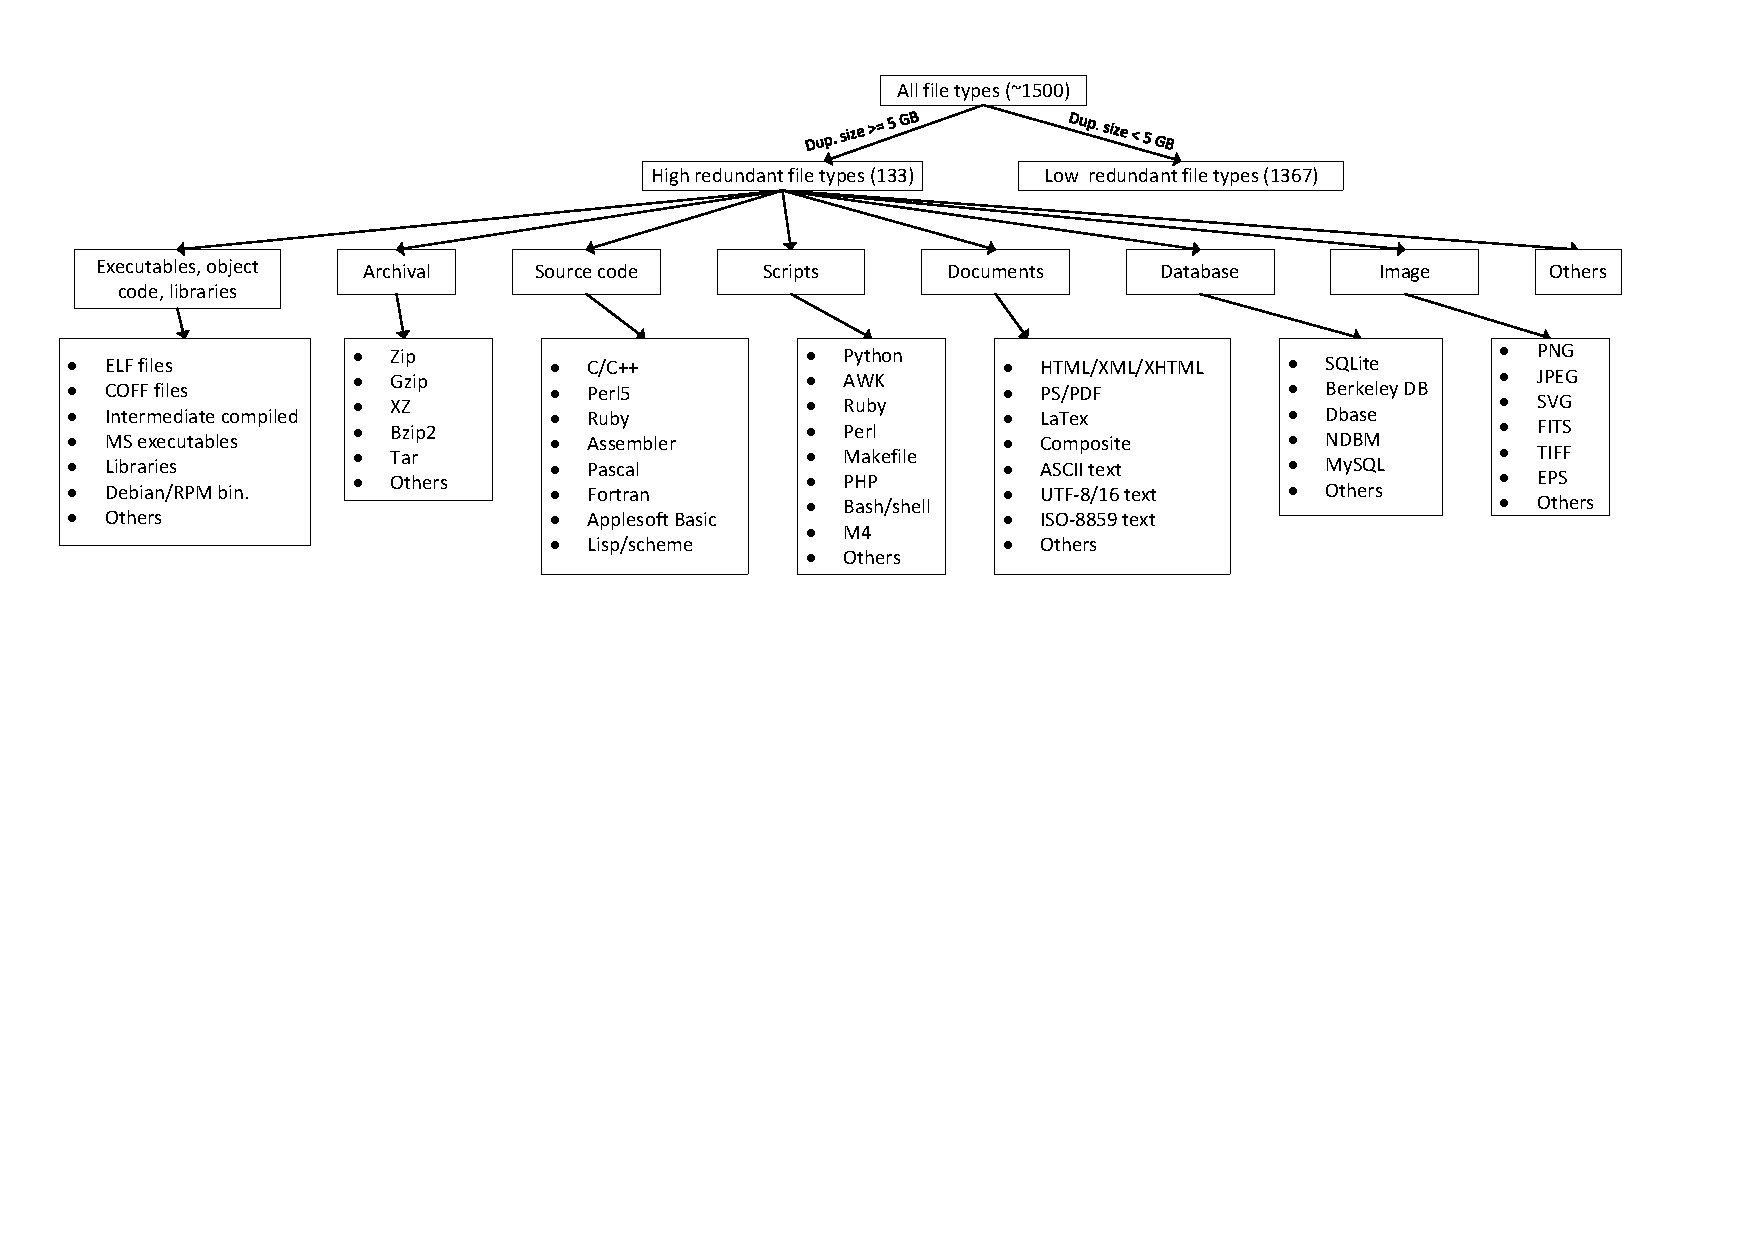
\includegraphics[width=1\textwidth]{graphs/graph-types-hierarchy}
	\caption{Taxonomy of file types.
	}
	\label{fig:file-type-hierarchy}
\end{figure*}

\paragraph{Common used file types}

\begin{figure}
	\centering
	\subfigure[File count (in \%) by file type group.]{\label{fig:type-total-cnt}
		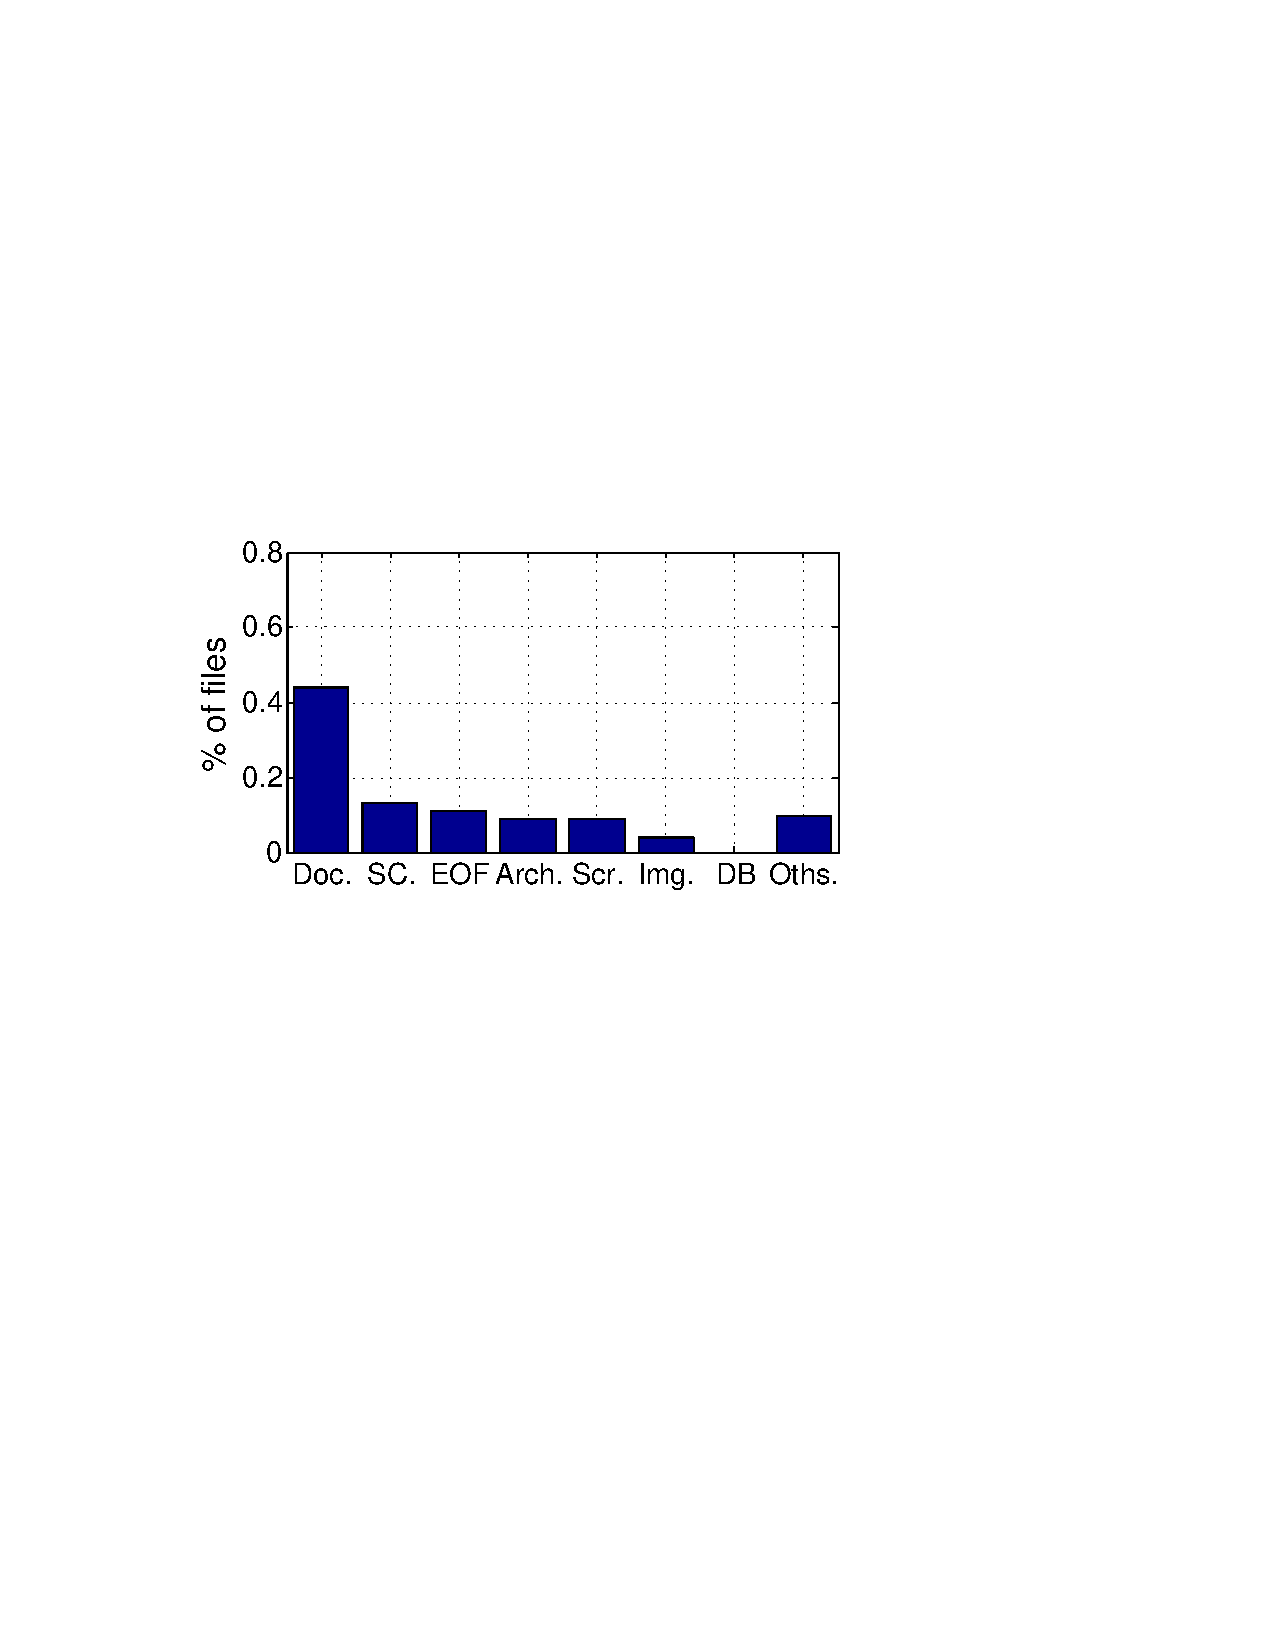
\includegraphics [width=0.225\textwidth]{graphs/type-total-cnt}
	}
	\subfigure[Capacity (in \%) by file type group.]{\label{fig:type-total-size}
		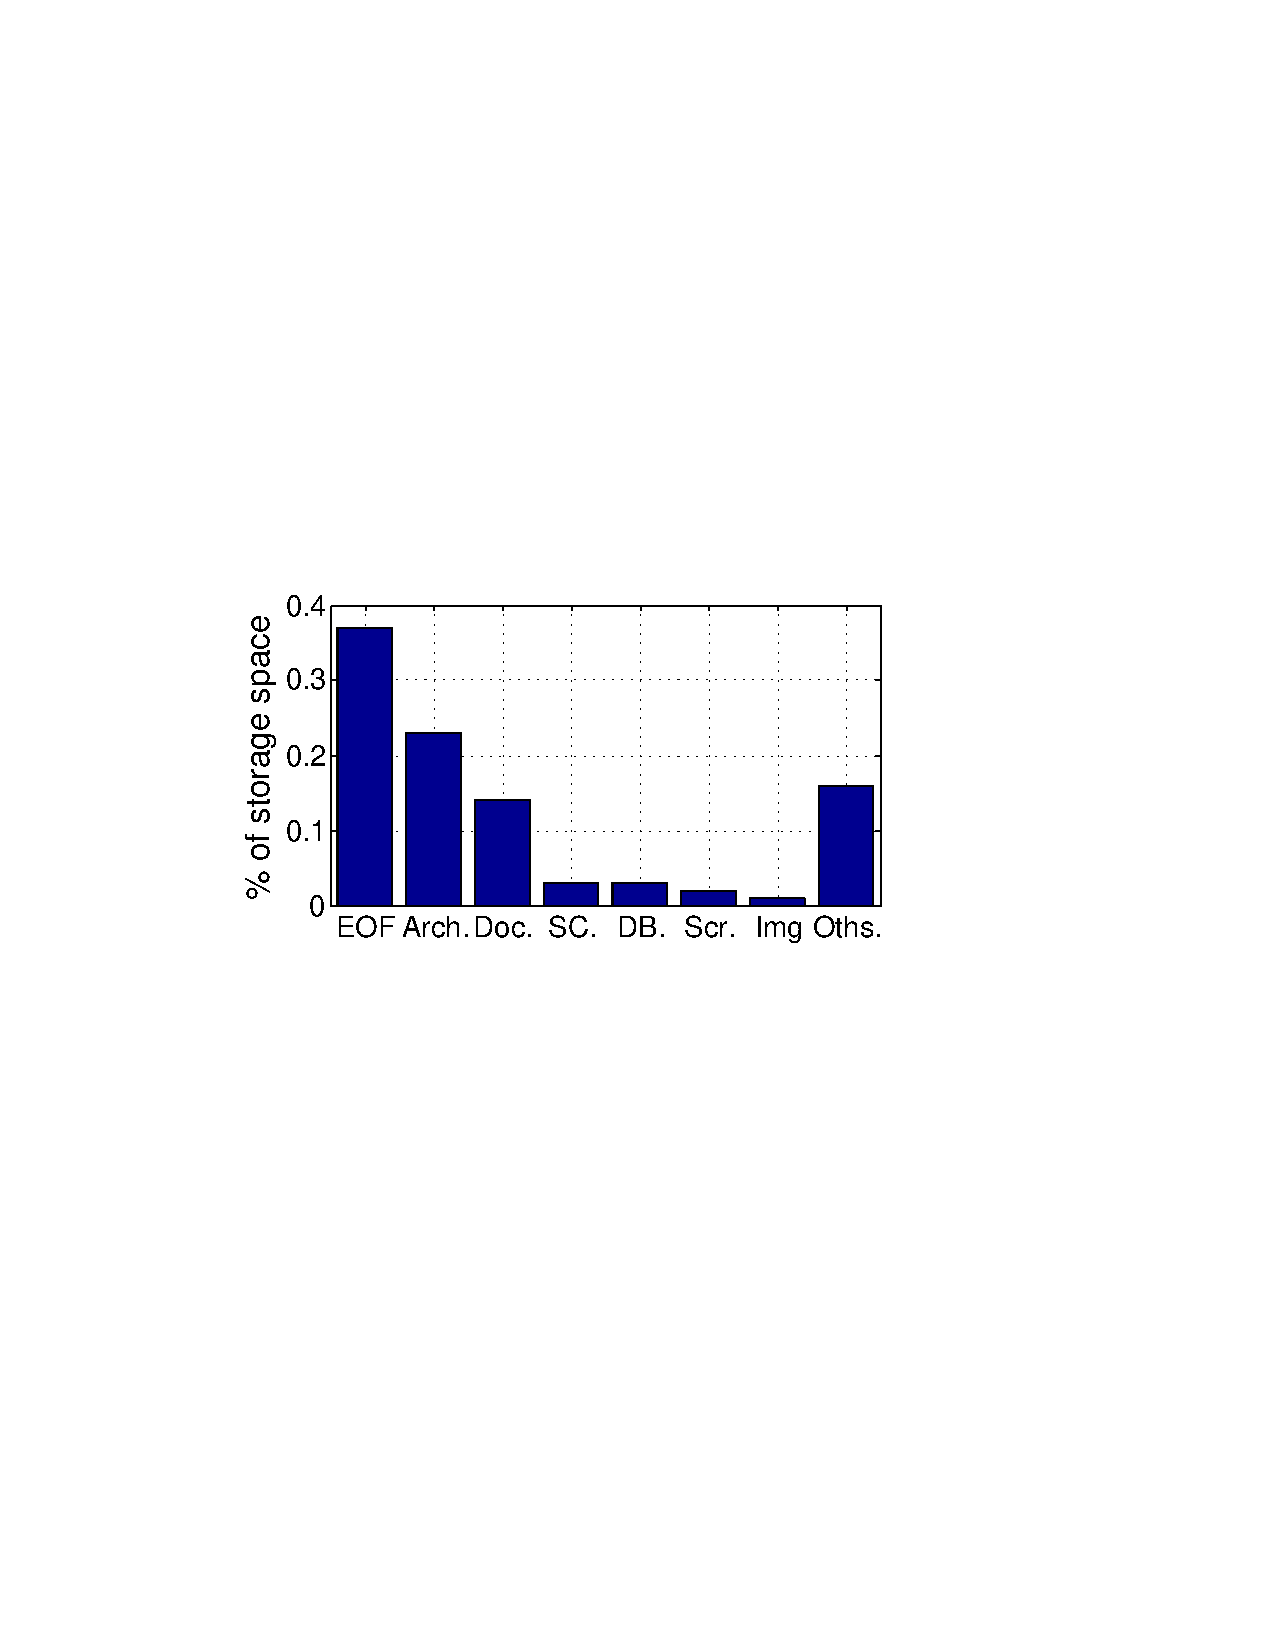
\includegraphics [width=0.225\textwidth]{graphs/type-total-size}
	}
	\caption{Common used file types}
	\label{fig:type-total}
\end{figure}

Figure~\ref{fig:type-total} shows the 8 type groups in terms of file count and capacity.  
13\%, 11\%, and 9\% of files are source code, EOL, and scripts. 
EOL occupy the most of capacity (37\%). 
We can infer that developers mostly use Docker to develop, build, and run applications. This finding align with that images package more source codes and binaries needed for runtime.

We also see that Docker developers conduct many other activities in addition to coding. 
For example, 44\% of files are documents that contains Microsoft office files, LaTex files, etc., which means that developers also composite documents in Docker containers. 4\% of files are image data files that contains PNG, JPEG, etc. Besides, we found small amount of video files, such as AVI, MPEG, etc., meaning that developers also process images or videos in Docker containers.

xxx~\cite{xxxx} shows that there is relation between file type and file size. 
To find how file type relate to file size, we calculated the average file size by file type group as shown in
Figure~\ref{fig:type-total-avg-size}. We see that Database files are much bigger (978.8 KB) than the files within other type groups. The average size of EOF and Archival files are around 100 KB. 
\textit{This finding is especially important for designer to optimize image size or mitigate registry storage overhead based on different file type}

%\begin{figure}
%	\centering
%	\subfigure[File count (in \%) by file type group.]{\label{fig:type-total-avg-size}
%		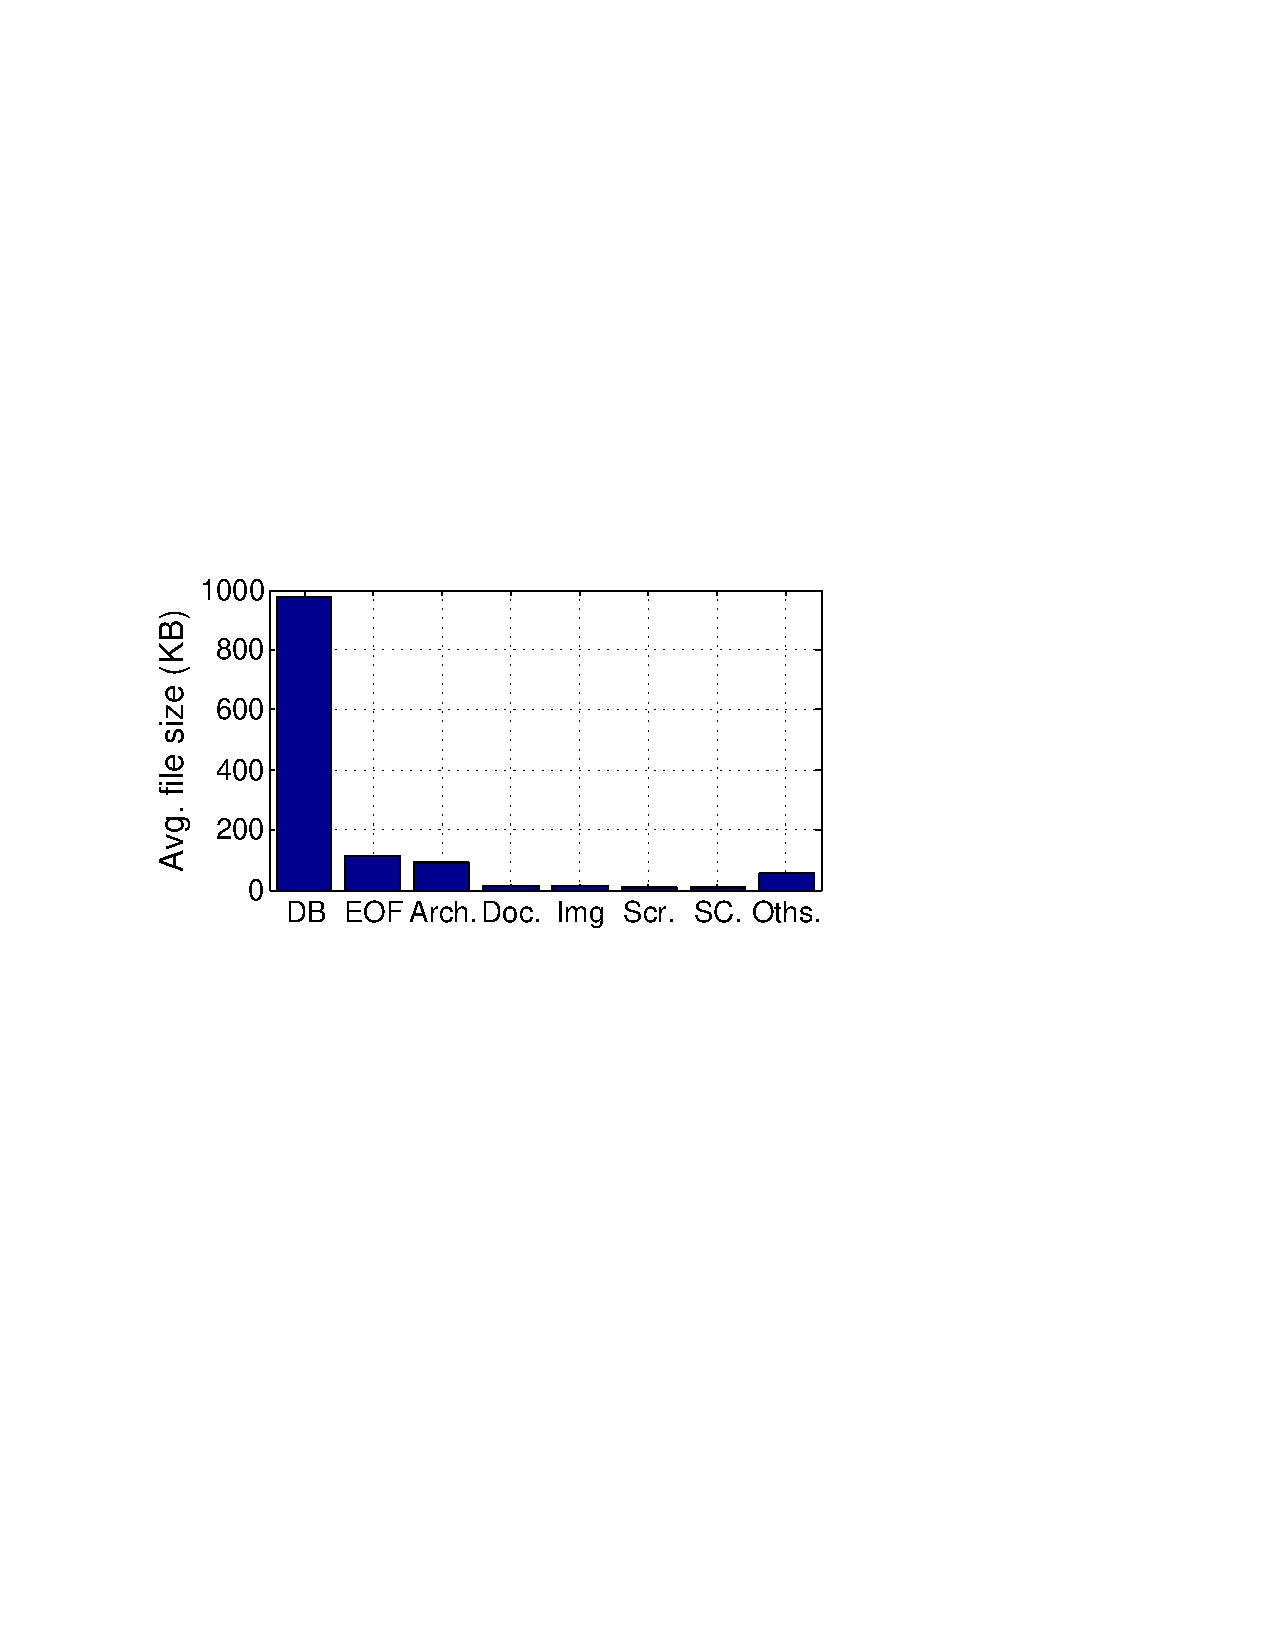
\includegraphics [width=0.225\textwidth]{graphs/type-total-avg-size}
%	}
%	\subfigure[Capacity (in \%) by file type group.]{\label{fig:type-total-size}
%		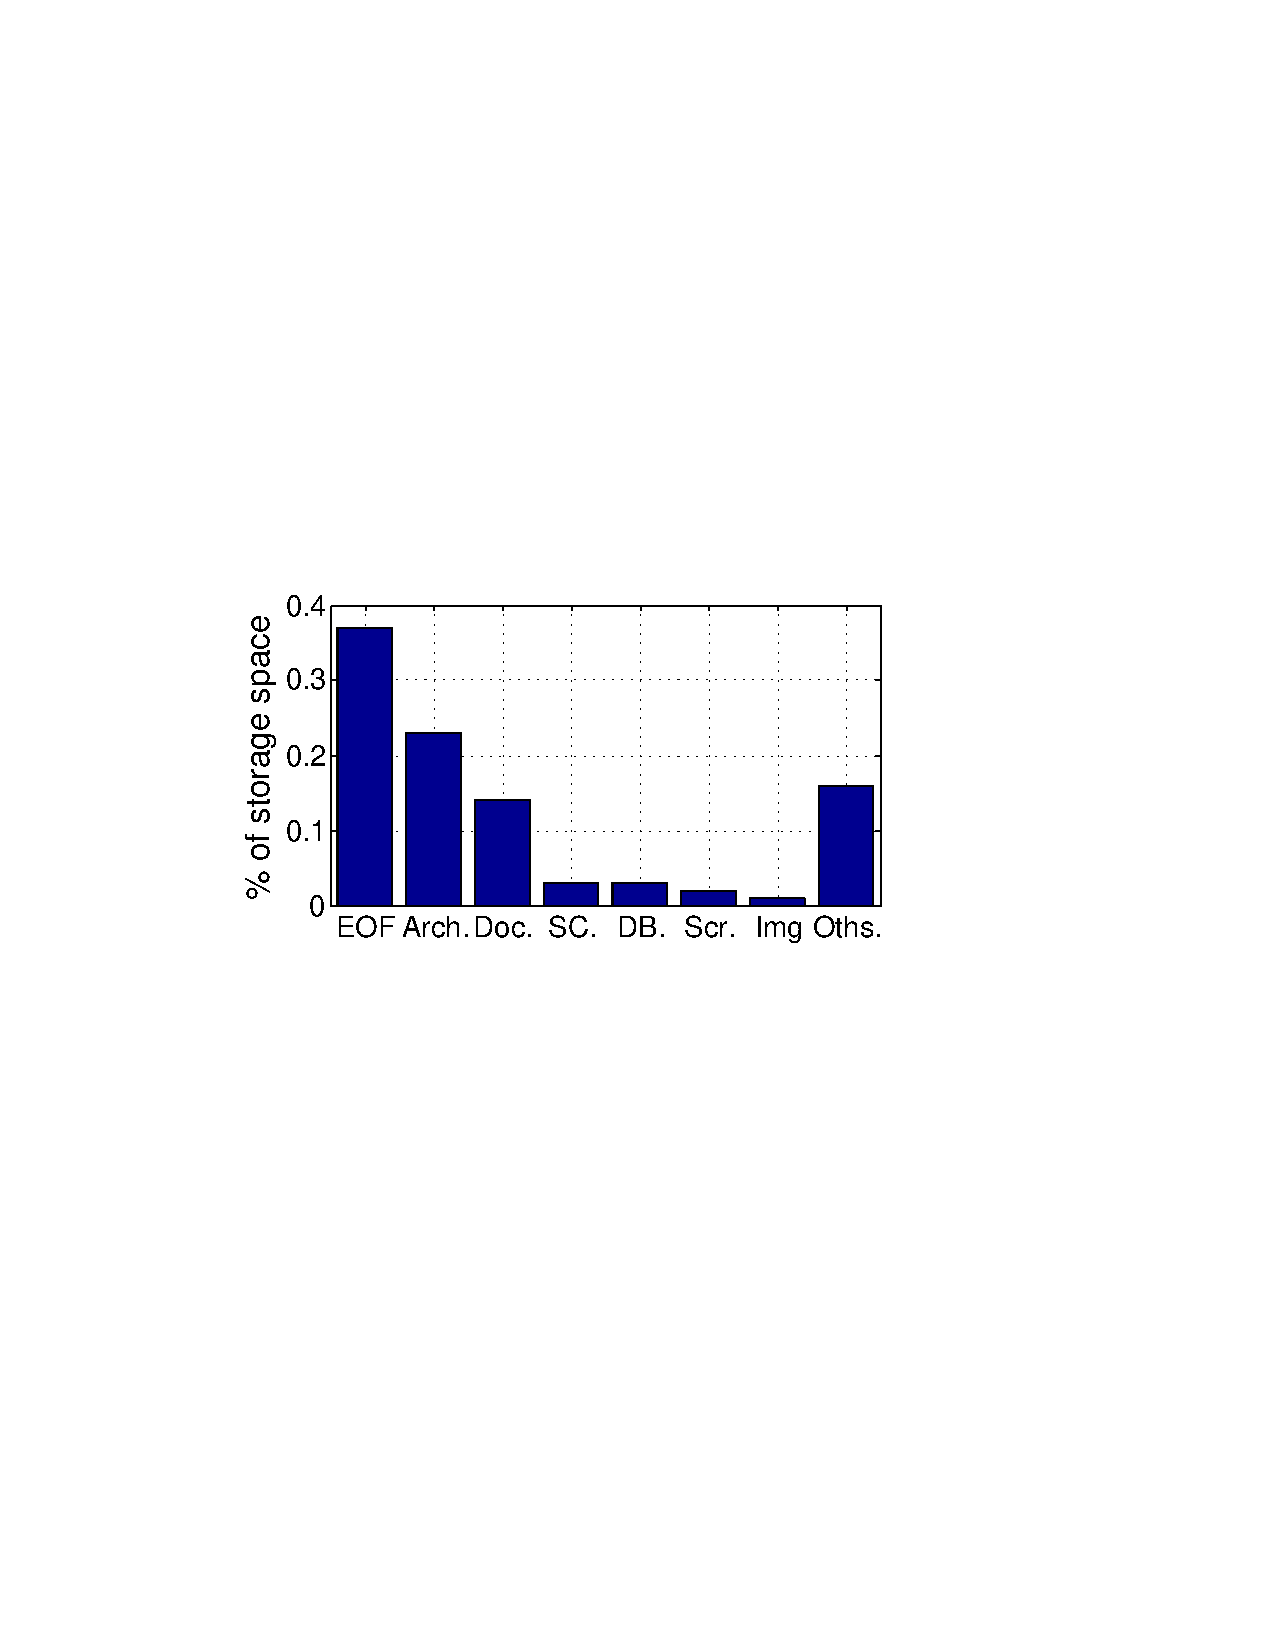
\includegraphics [width=0.225\textwidth]{graphs/type-total-size}
%	}
%	\caption{Common used file types}
%	\label{fig:type-total-size}
%\end{figure}

\begin{figure}[!t]
	\centering
	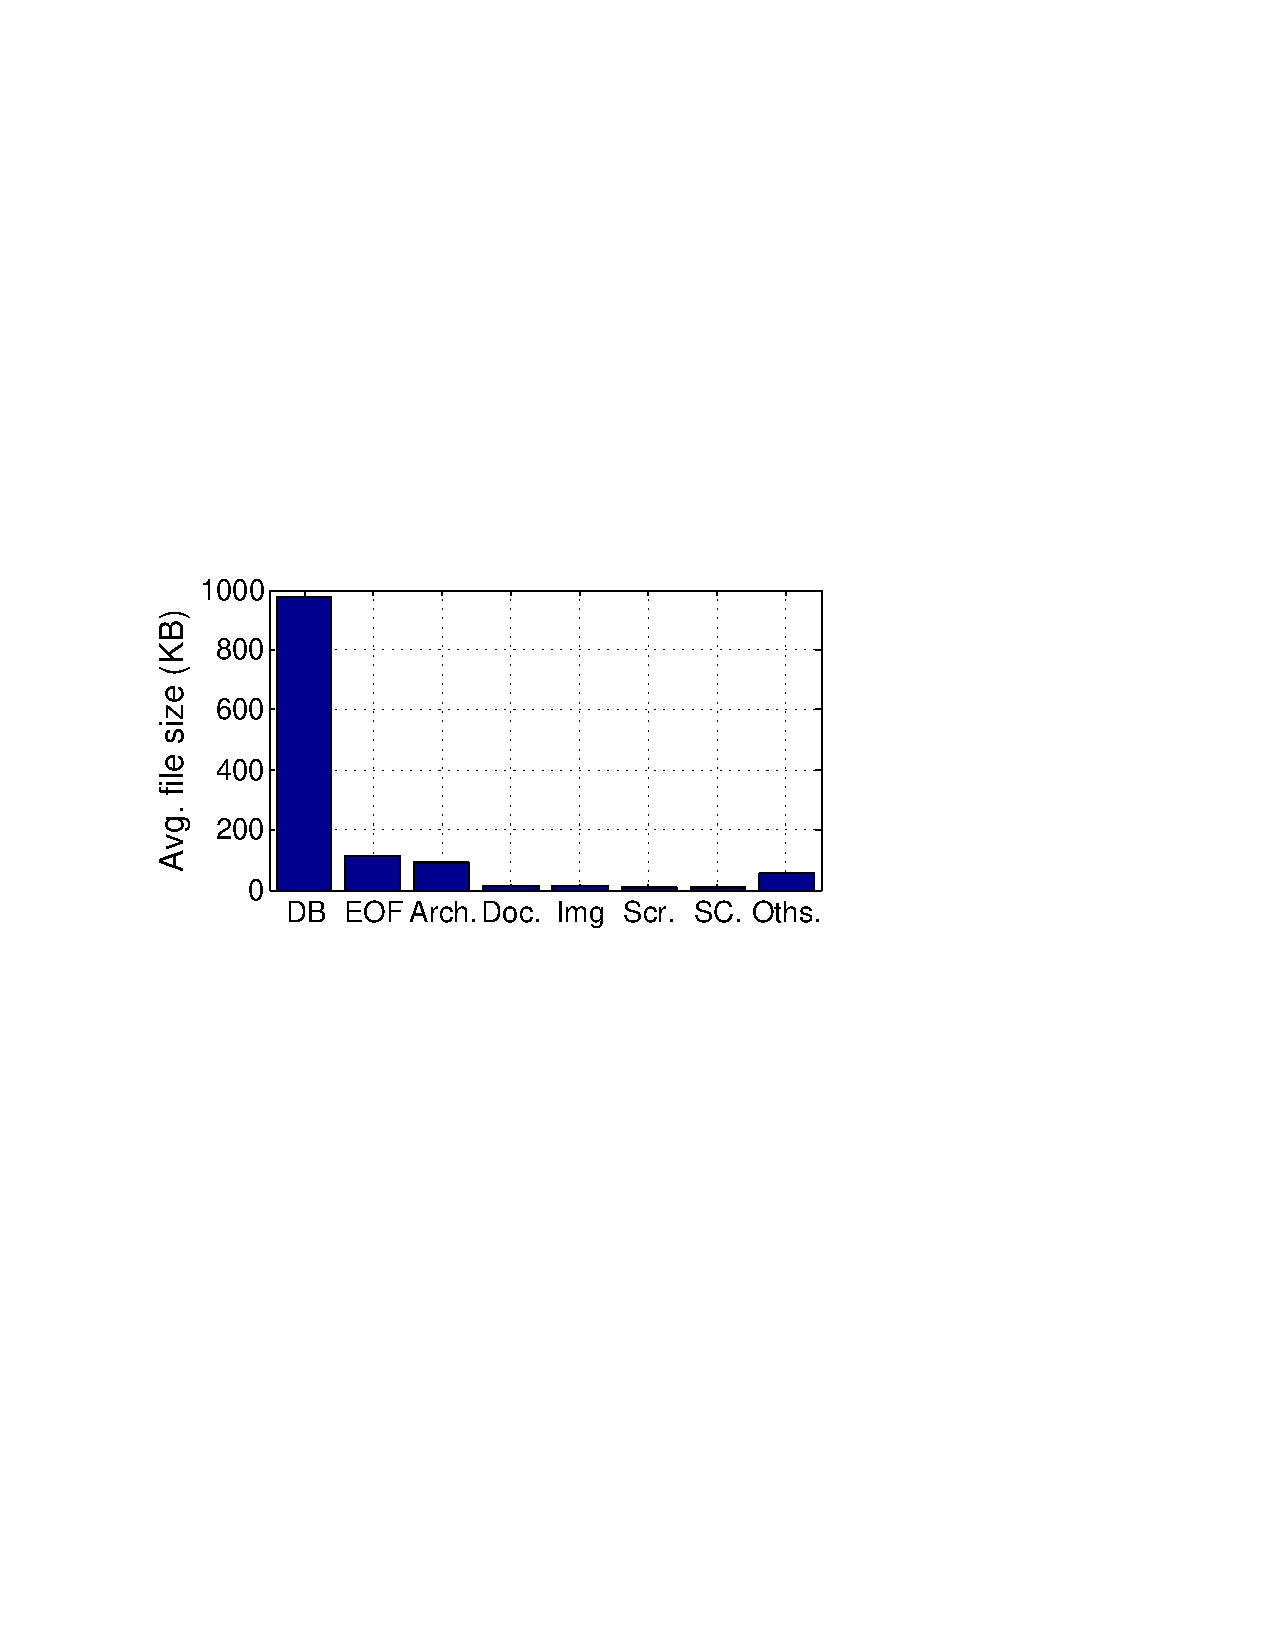
\includegraphics [width=0.225\textwidth]{graphs/type-total-avg-size}
	\caption{Average file size by file type group.}
	\label{fig:type-total-avg-size}
\end{figure}

% or further classify the redundant files based on involved by each file type. 
%We selected the file types which take largest storage space.

\paragraph{Executable, object code, and libraries (EOL)}
Based on the second-and third-classification, we further investigate the file size and file count by specific file types. We first start with EOF type group which contains the following types: ELF files, COFF files, intermediate representation that can be executed by virtual machine, Microsoft executables, Debian/RPM binary packages, libraries, and other EOF files.

Figure~\ref{fig:type-eof} shows file type distribution in terms of file count and capacity for EOL type group. 
We see that majority of EOL files are ELF and intermediate representations. ELF files mainly contains ELF relocatable, shared object, and executables. Intermediate representations mainly contains Python Byte-compiled files (majority), compiled java class, and terminfo compiled files. Although intermediate representations take up to 64\% of EOL files, 30\% of EOL files occupy 84\% of storage space consumed by EOL group. 
This is because average ELF file size is 312.7 KB while average intermediate compiled file size is 9 KB. In addition to ELF files and representations, we found Microsoft executables (2\%) and Mach-O files ($<$0.01\%) in the EOL type group.

\textit{We conclude that among all file types, ELF files occupy most capacity. There are large amount of intermediate representations but they take very less storage space.}

\begin{figure}
	\centering
	\subfigure[File count (in \%) by file type.]{\label{fig:type-eof-cnt}
		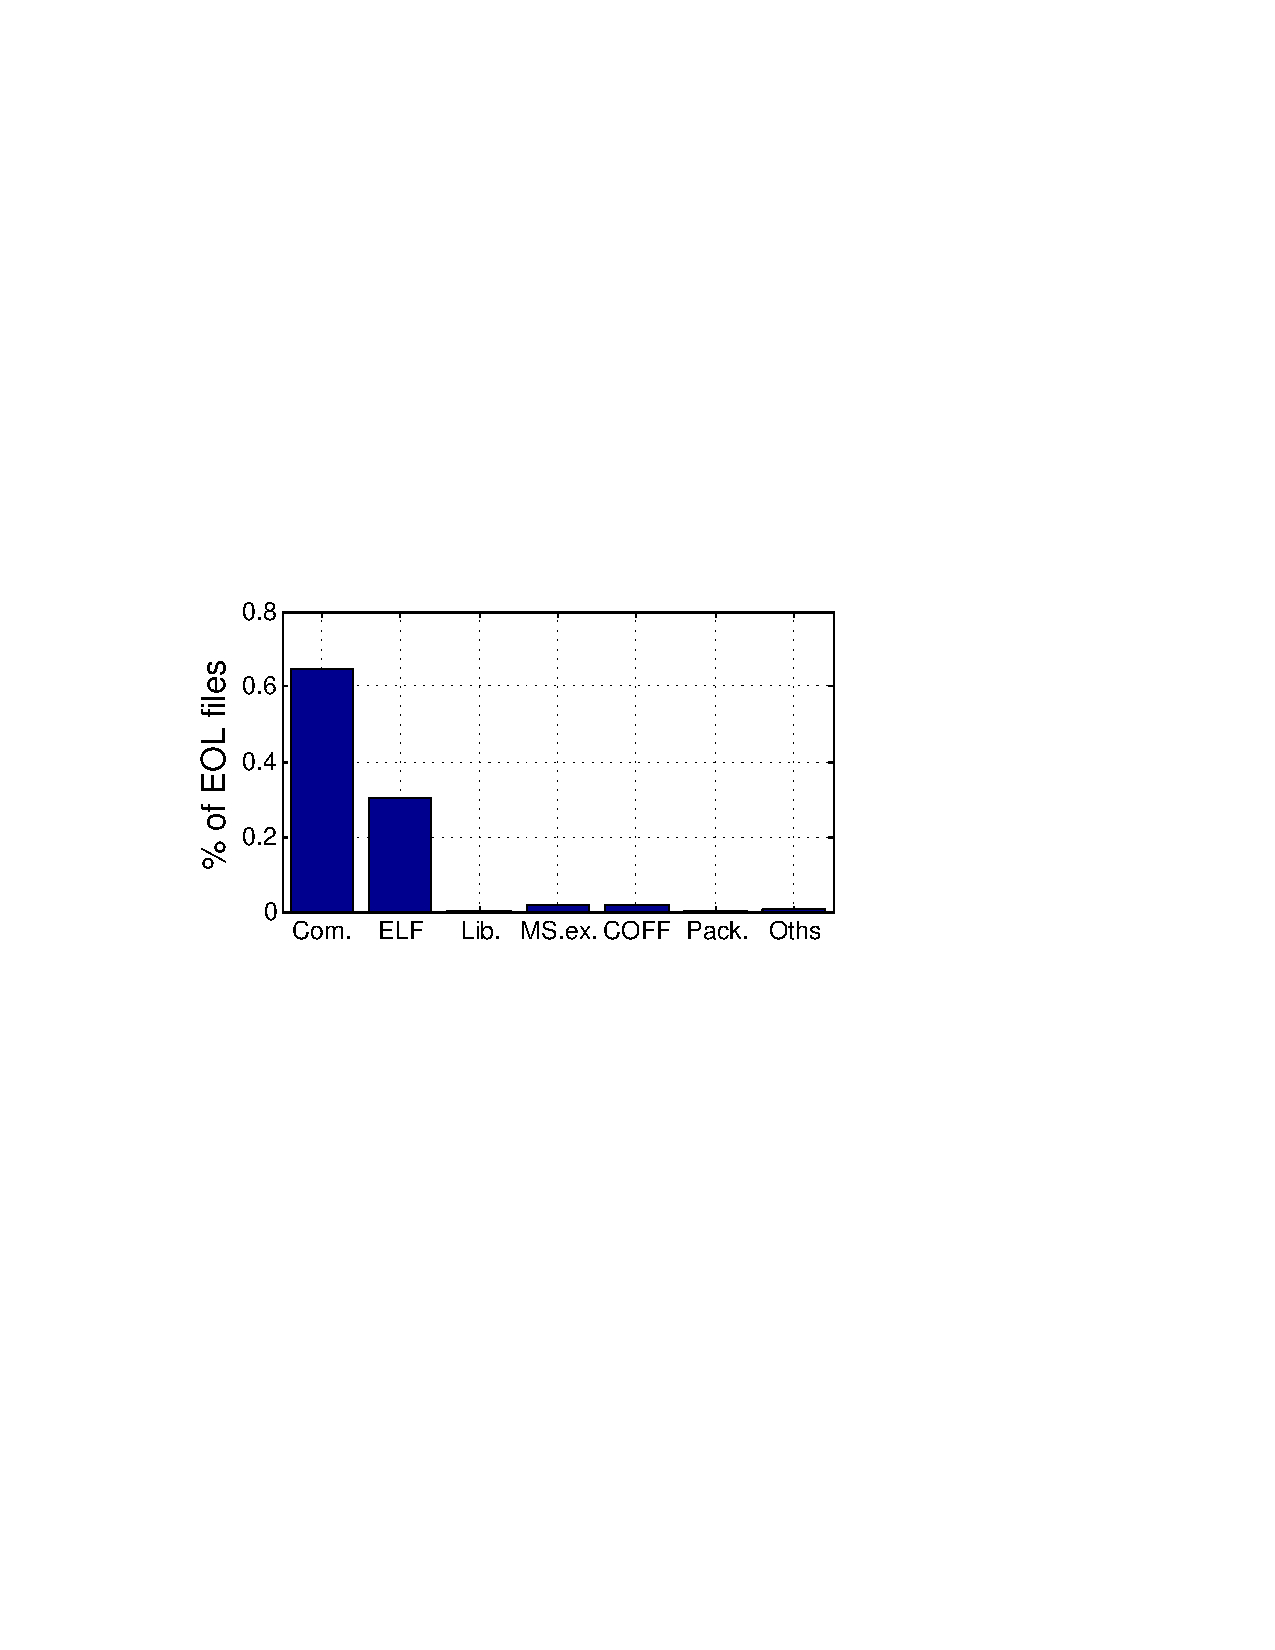
\includegraphics [width=0.225\textwidth]{graphs/type-eof-cnt}
	}
	\subfigure[Capacity (in \%) by file type.]{\label{fig:type-eof-size}
		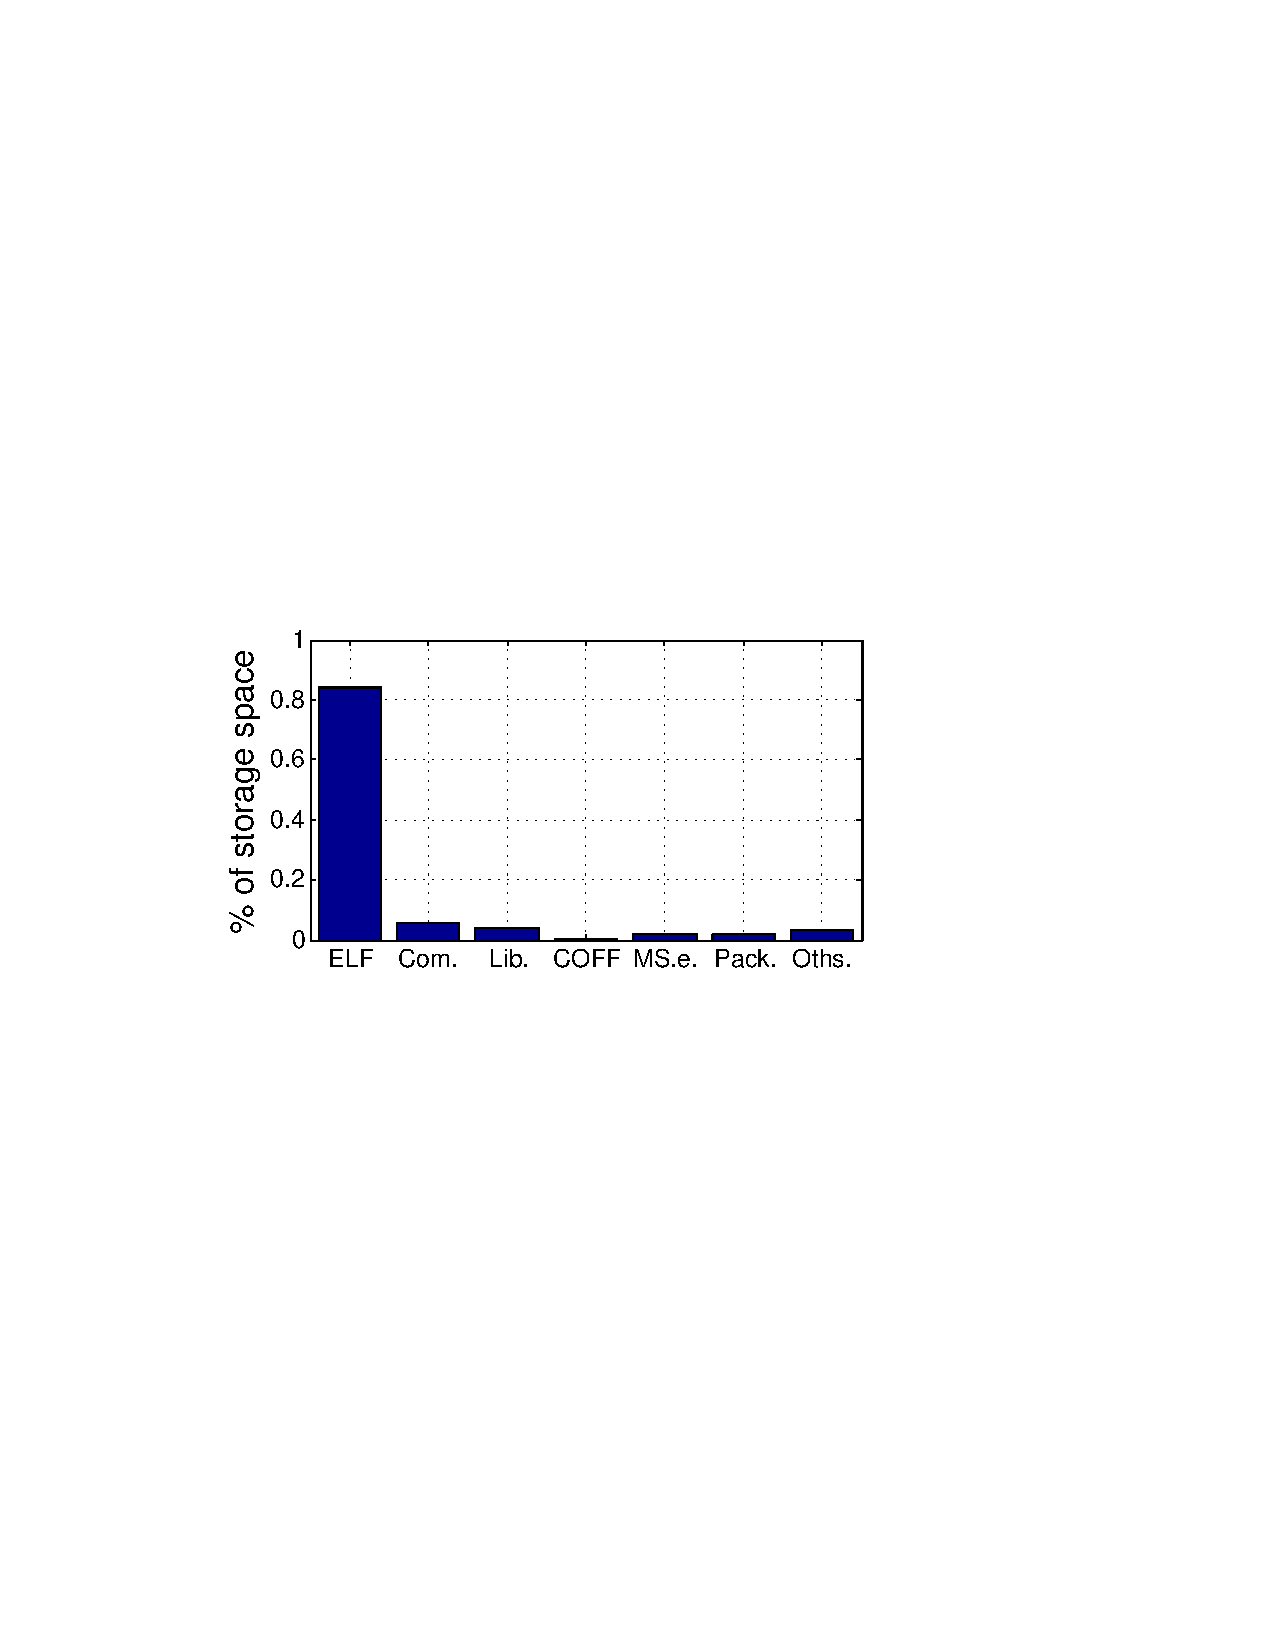
\includegraphics [width=0.225\textwidth]{graphs/type-eof-size}
	}
	\caption{EOL files}
	\label{fig:type-eof}
\end{figure}

\begin{figure}
	\centering
	\subfigure[File count (in \%) by file type.]{\label{fig:type-sc-cnt}
		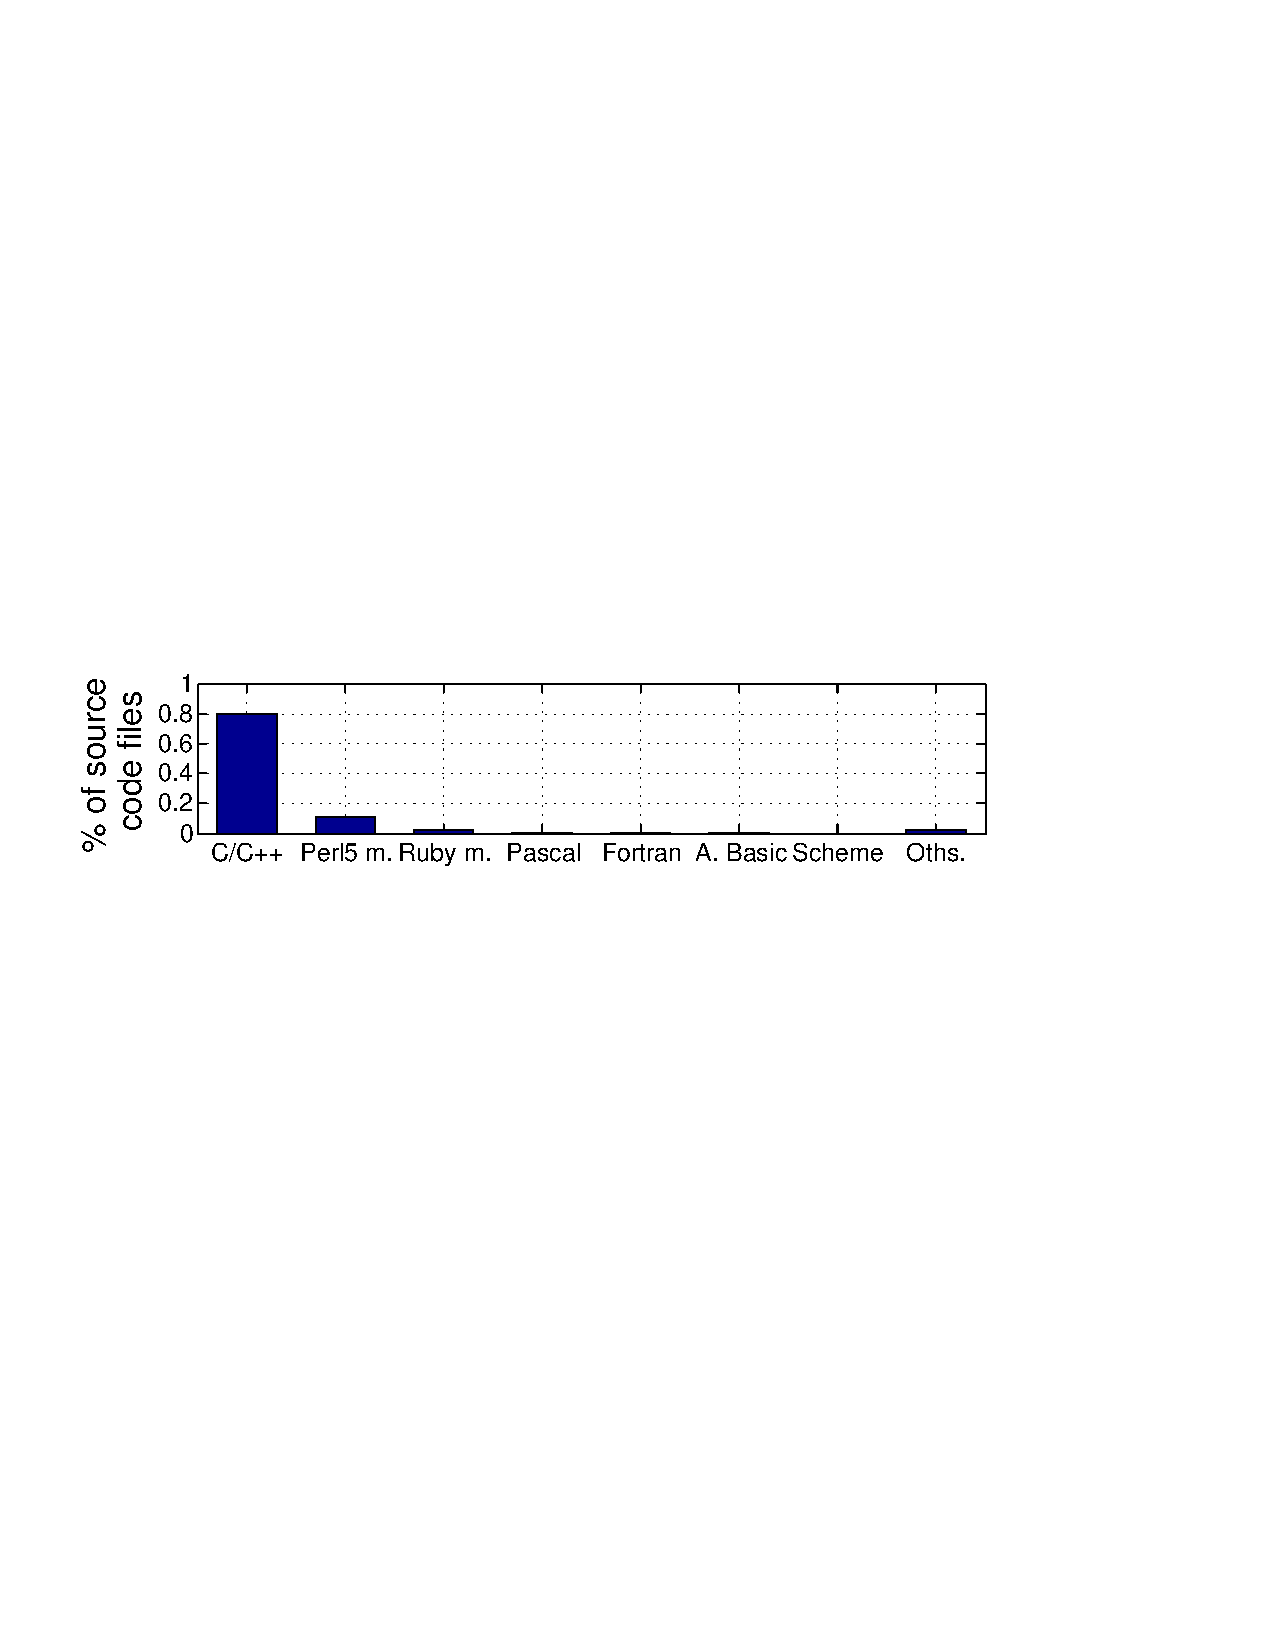
\includegraphics [width=0.4\textwidth]{graphs/type-sc-cnt}
	}
	\subfigure[Capacity (in \%) by file type.]{\label{fig:type-sc-size}
		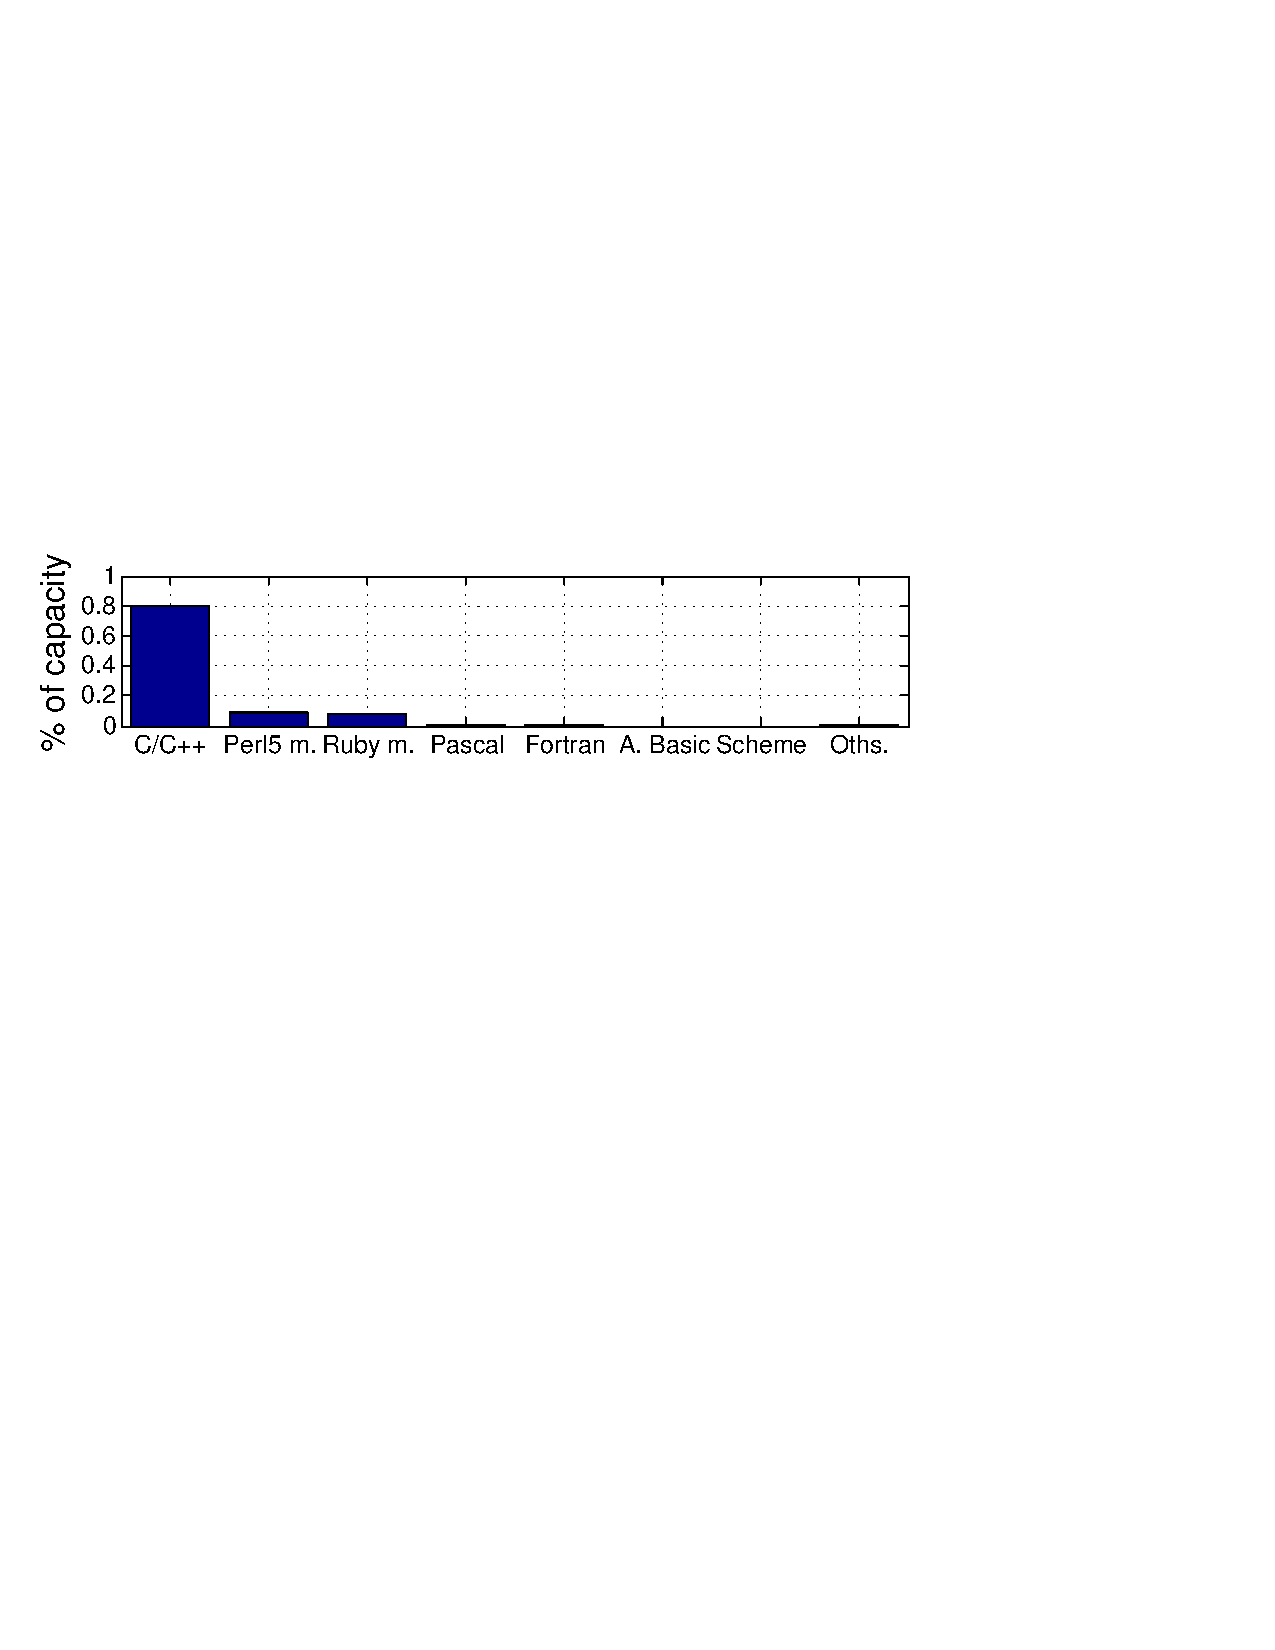
\includegraphics [width=0.38\textwidth]{graphs/type-sc-size}
	}
	\caption{Source codes}
	\label{fig:type-sc}
\end{figure}

\begin{figure}
	\centering
	\subfigure[File count (in \%) by file type.]{\label{fig:type-scrp-cnt}
		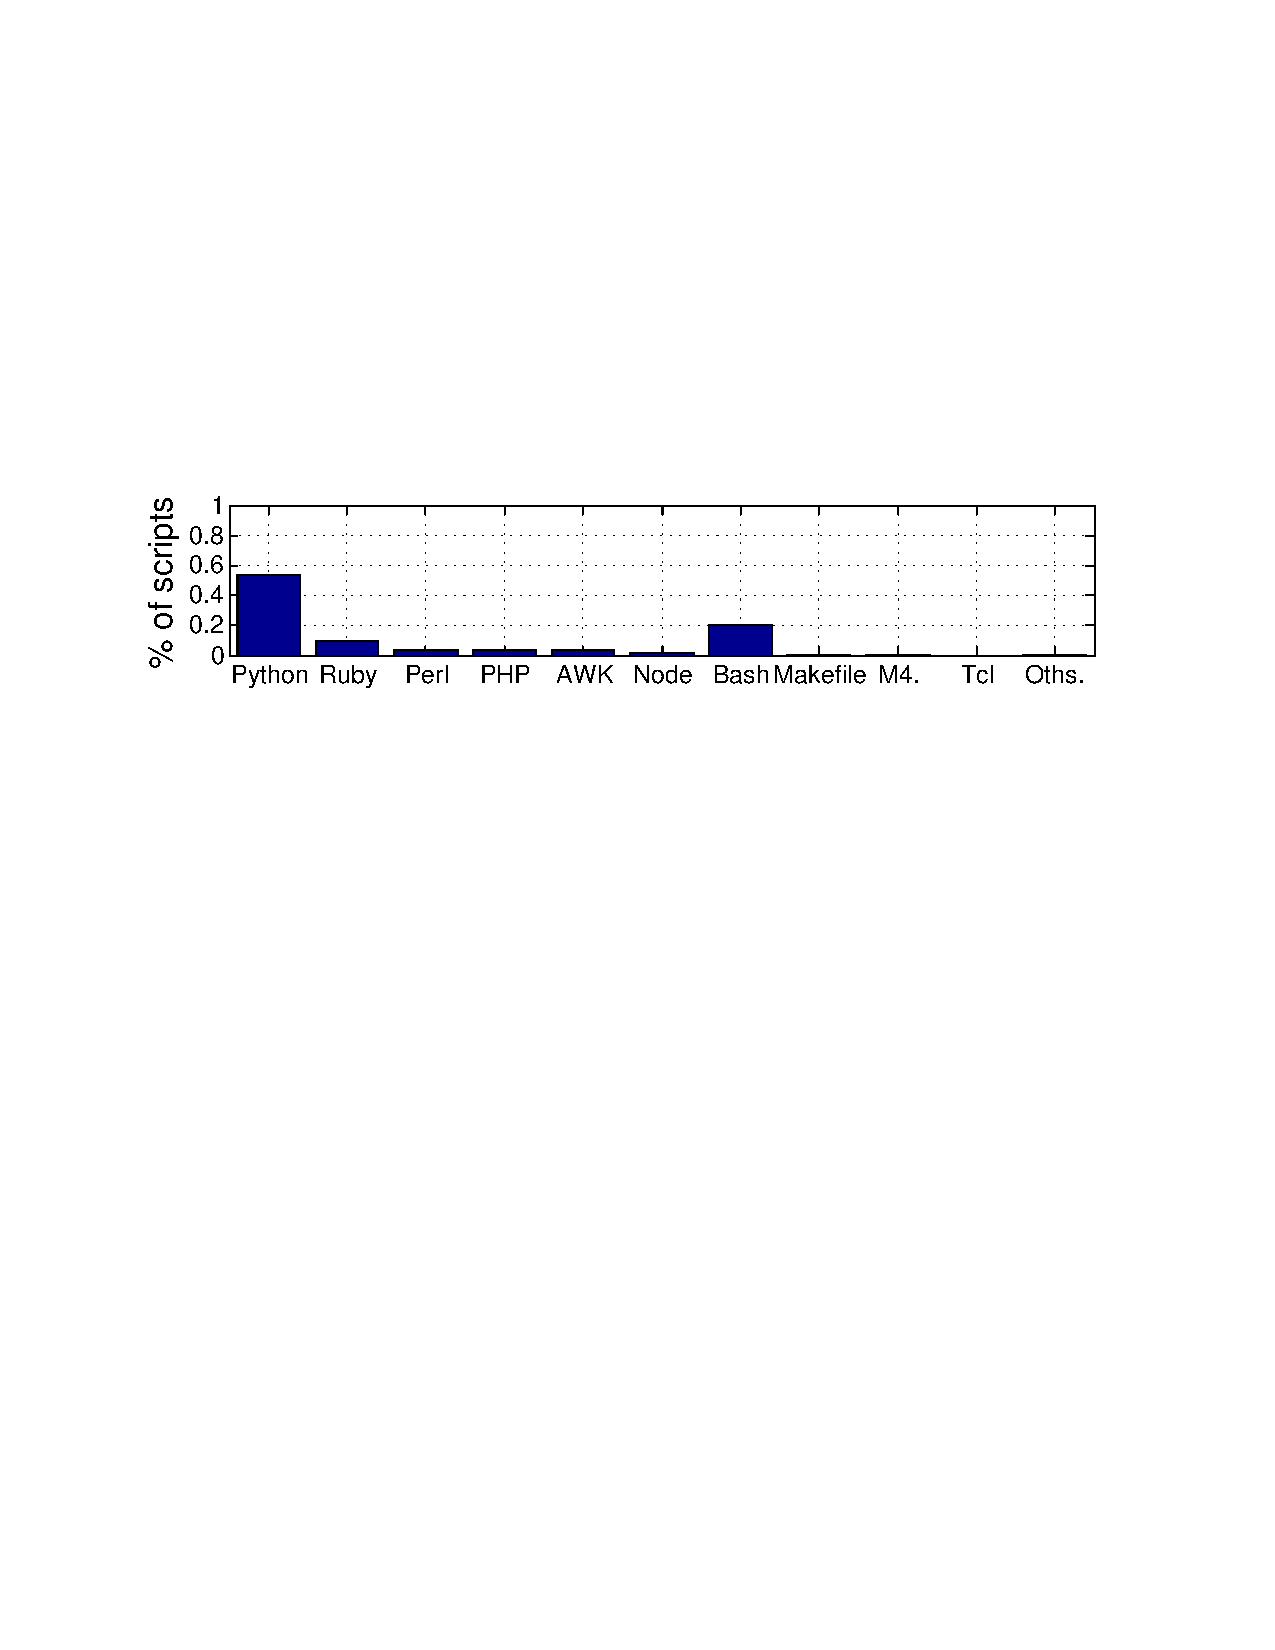
\includegraphics [width=0.4\textwidth]{graphs/type-scrp-cnt}
	}
	\subfigure[Capacity (in \%) by file type.]{\label{fig:type-scrp-size}
		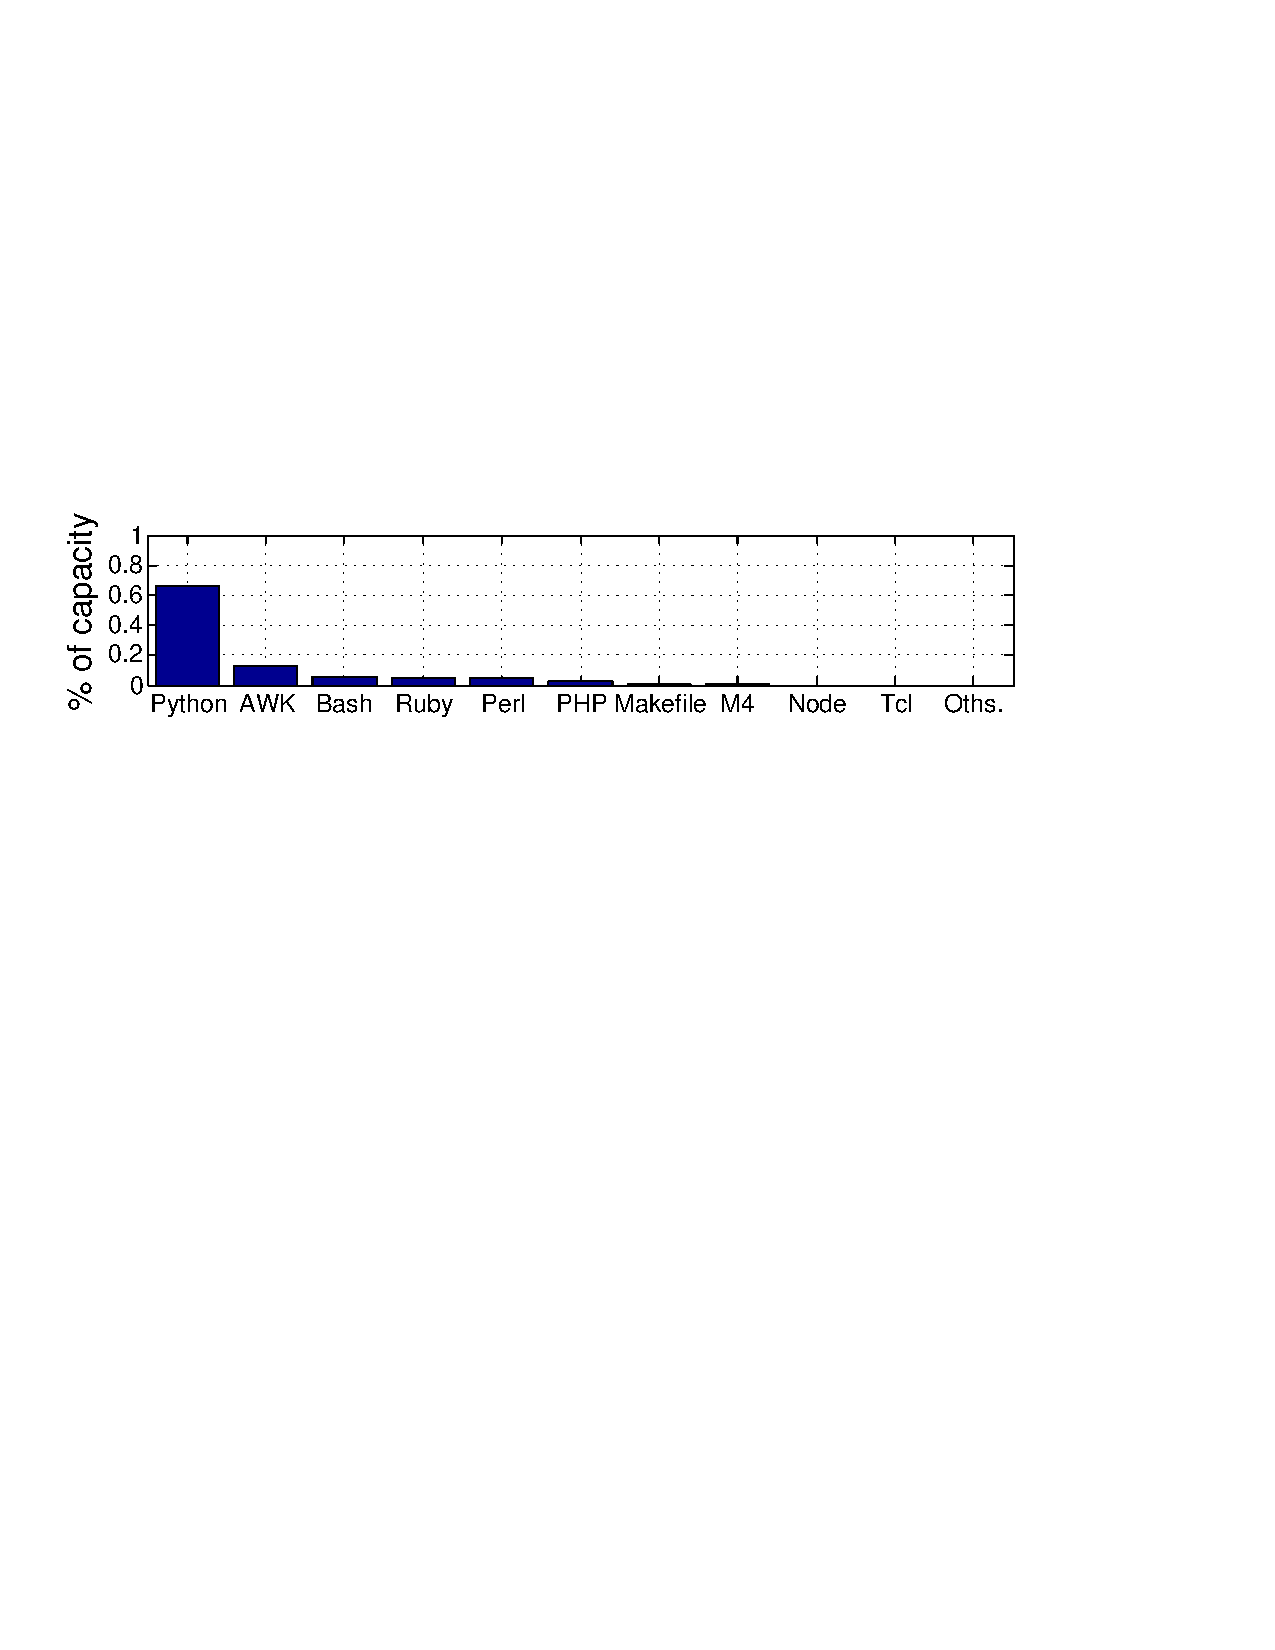
\includegraphics [width=0.4\textwidth]{graphs/type-scrp-size}
	}
	\caption{Scripts}
	\label{fig:type-script}
\end{figure}

\begin{figure}
	\centering
	\subfigure[File count (in \%) by file type.]{\label{fig:type-doc-cnt}
		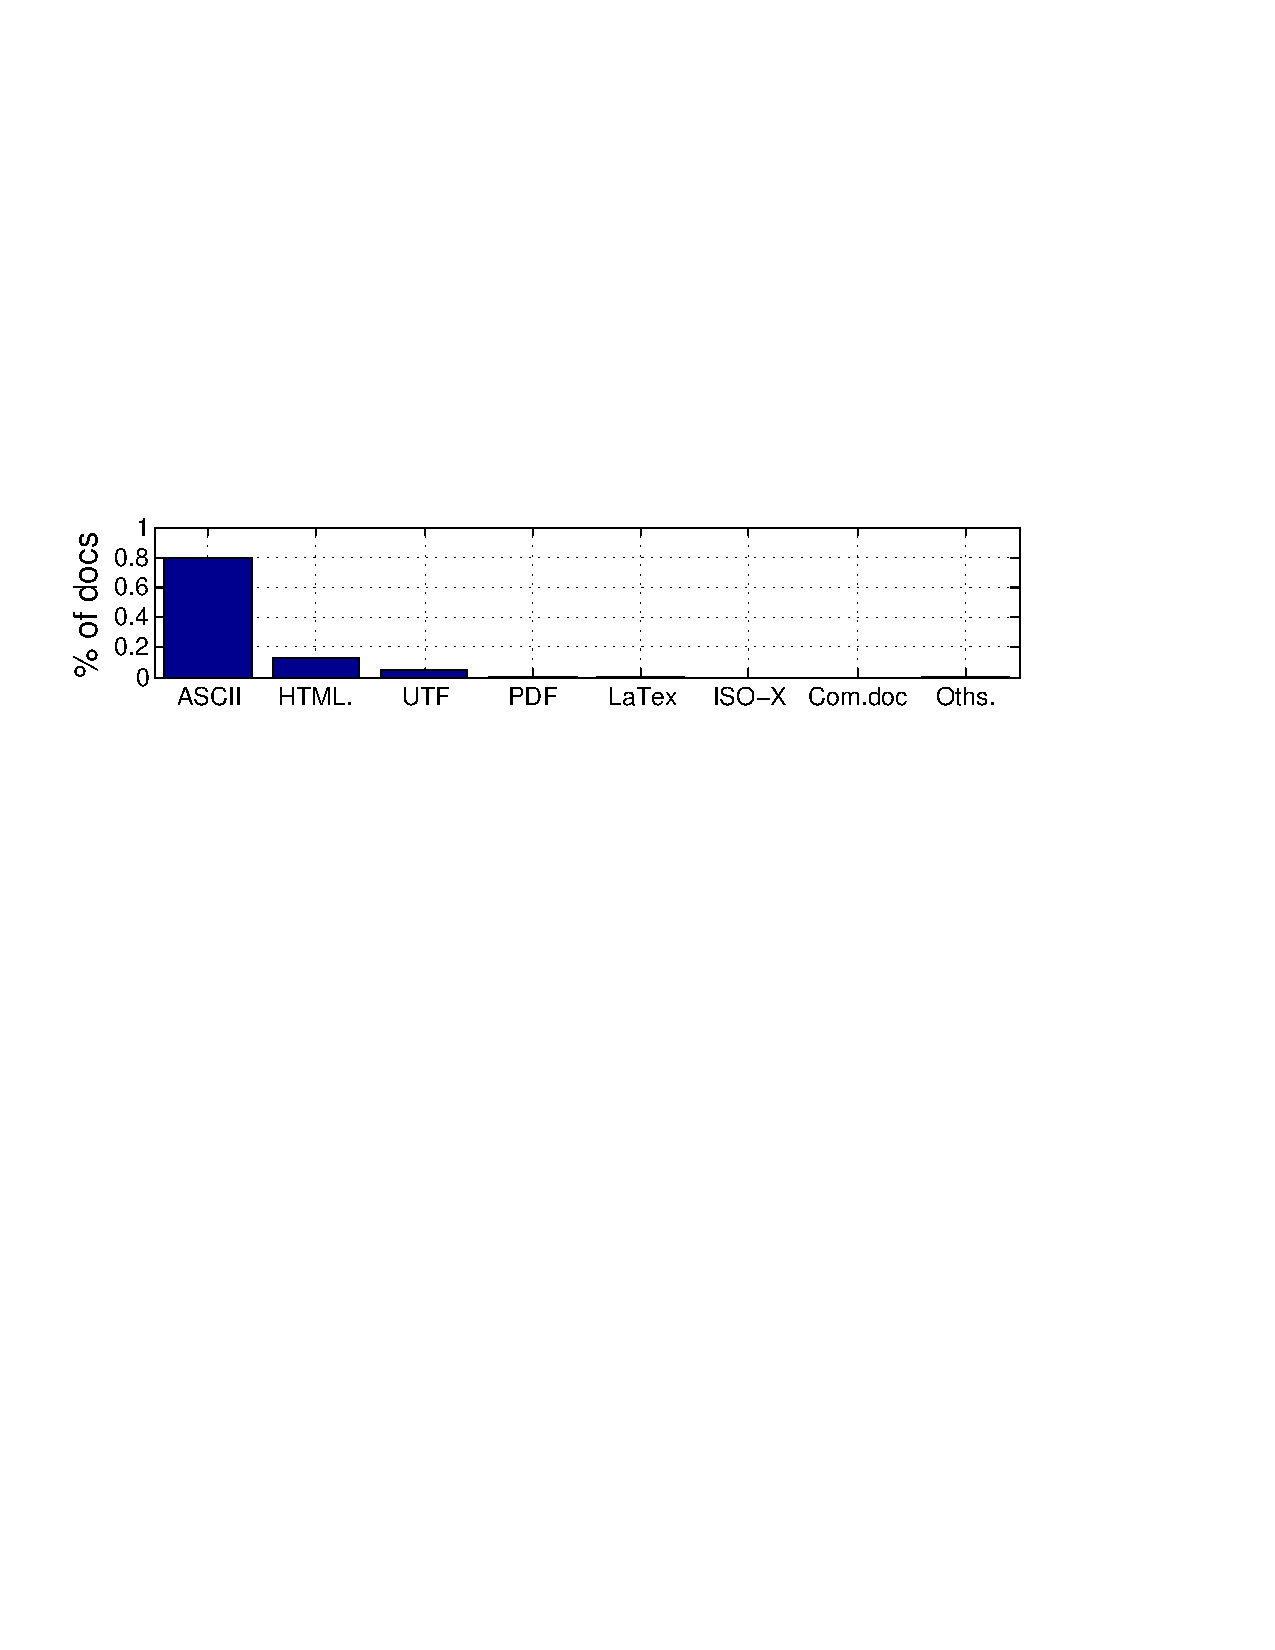
\includegraphics [width=0.4\textwidth]{graphs/type-doc-cnt}
	}
	\subfigure[Capacity (in \%) by file type.]{\label{fig:type-doc-size}
		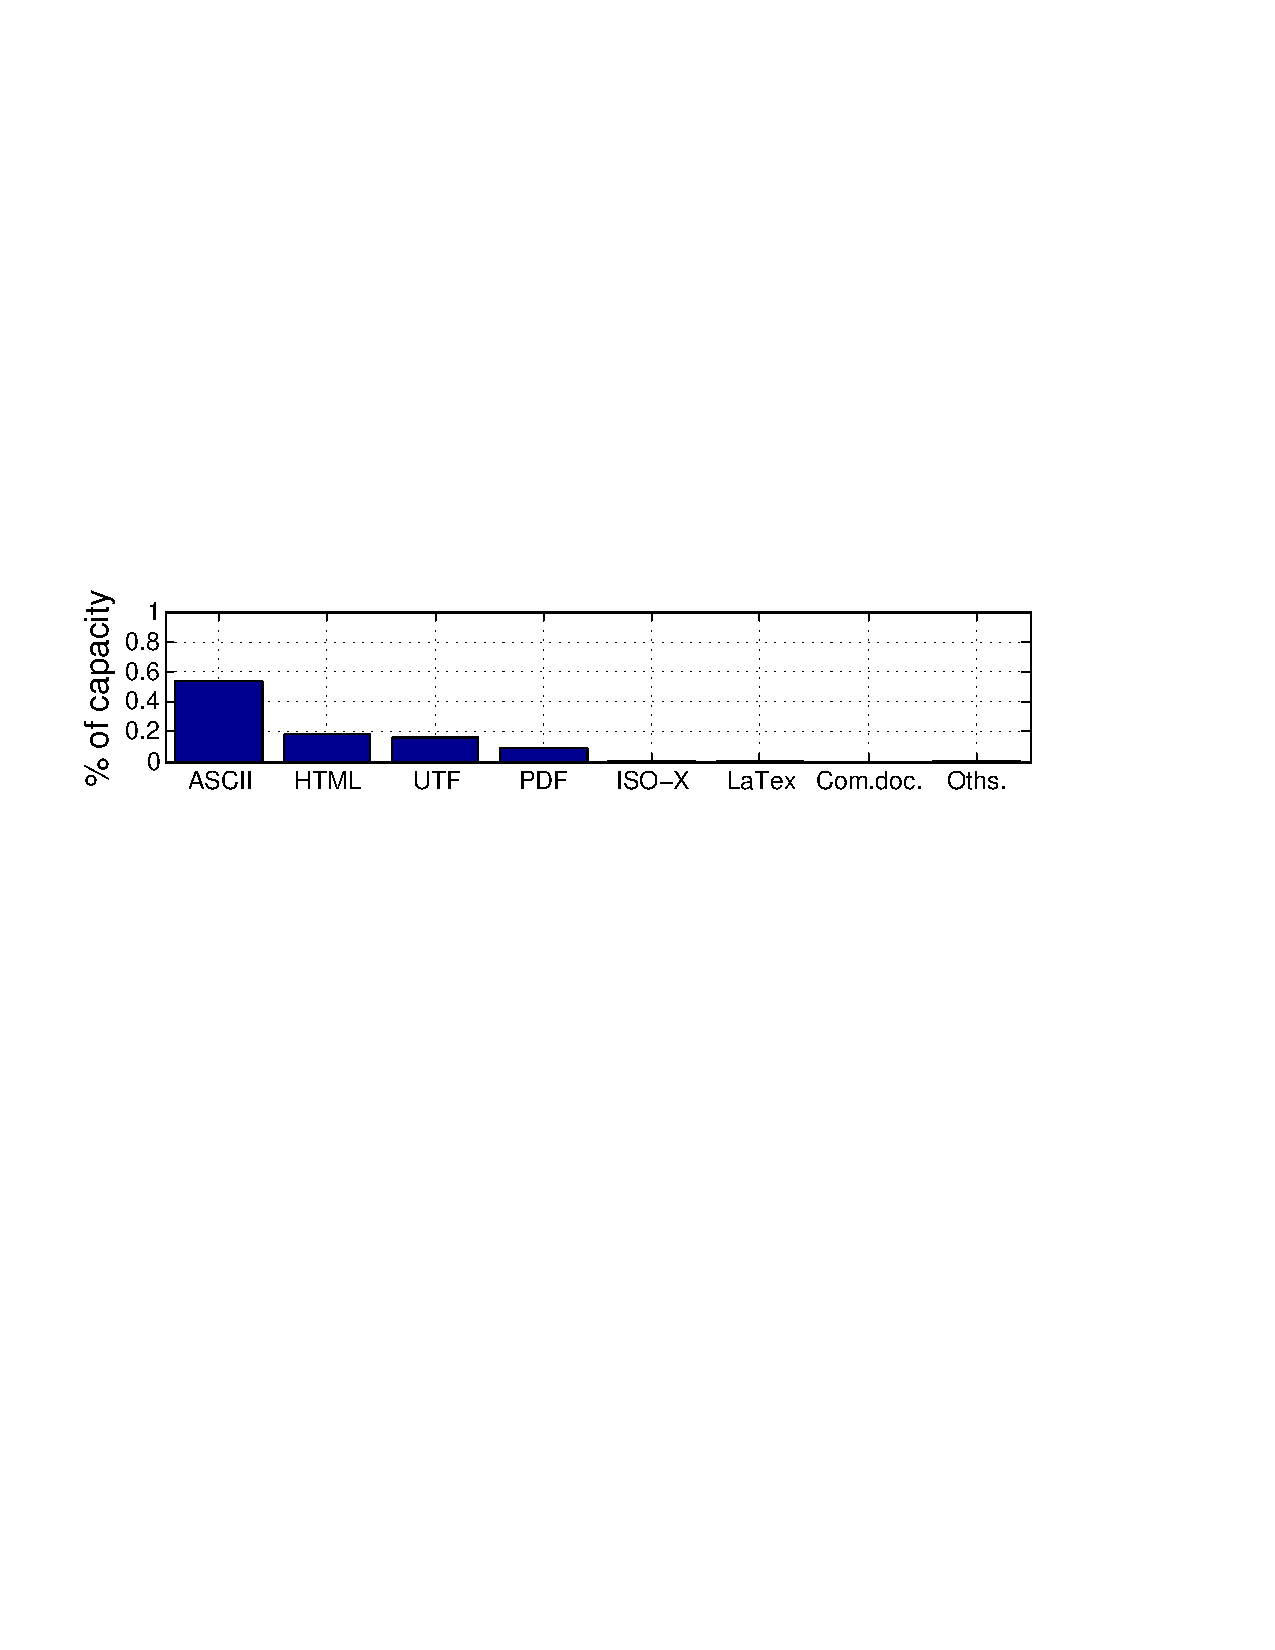
\includegraphics [width=0.4\textwidth]{graphs/type-doc-size}
	}
	\caption{Documents}
	\label{fig:type-doc}
\end{figure} 


%We also find 0.2\% of EOL files are libraries, which contains 
 
% meaning that developers also use other operating systems in addition to Linux, such as Windows and mac OS.
 
To know what kind of libraries are used in Docker containers, we categorized the libraries and found the following major libraries: Palm OS dynamic library, OCaml library, and GNU C libraries. 
%\textit{}
\textit{We can see that developers conduct a diversity developments on different operating systems, such as Linux/Unix, macOS, Windows, and other operating systems for smart devices by using different programing languages.} 
%also an important files for Docker developer
\paragraph{Source code (SC.)}
Next, we inspect what kind of languages are commonly used by Docker developer. 
Figure~\ref{fig:type-sc} shows 7 major types of source codes in our dataset: C/C++ source, Perl5 module source, Ruby module source, Pascal source, Fortran program, Applesoft basic program, Lisp/scheme program.
80.3\% of source codes are C/C++ source codes which take up to 80\% of storage space occupied by source codes. Perl5 module source code and Ruby module source code have almost similar percentage in terms of file count (9\% for Perl5 module source and 8\% for Ruby module source) while slightly different percentage in terms of capacity (11\% for Perl5 module source and 3\% for Ruby module source).

\textit{We conclude that C/C++ is the most commonly used programming language by Docker developers. In addition to C/C++, some developers also wrote small amount of codes in other different languages.}


\paragraph{Scripts (Scr.)}
Scripting languages are common used high-level programing languages since they operate at a high level of abstraction. Compare to source codes, we found more different types of scripts. 
Our script type group includes Python script, AWK script, Ruby script, Perl script, PHP script, Makefile script, M4 macro processor script, node script, Tcl script, Bash/shell script, and other scripts.
We see that more than half of scripts are Python script (53.5\%), which take up to 66\% of storage space occupied by all scripts. Another common used script is Bash/shell script (20\%) which only occupy 6\% of storage space occupied by all scripts. 10\% of scripts are Ruby scripts which takes up to 5\% of storage space occupied by all scripts. %AWK script and Perlstorage space occupied by all scripts
%4\%, 10\%, 
%There are plenty of AWK scripts (4\%) which take up over 12.8\% of storage space 

\textit{We conclude that Python script is the most commonly used scripting language by Docker developers. This finding is consistent with that Python Byte-compiled files are the major intermediate representations.
	In addition to Python, Docker developers also use other types of scripts.}

\paragraph{Documents (Doc.)}
As discussed before, 44\% of files are documents which take up to 14\% of storage space. So it's important to know what kinds of documents Docker developers create and store in Container. 
As shown in Figure~\ref{fig:type-doc}, we see that majority of documents are text files including ASCII text (80\%), UTF8/16 text (5\%), and ISO-8859 text (0.4\%), which take up to 70\% of storage space occupied by documents. Note that these text files are \textit{raw text files} since we already filter the text based well-known file types%applications
, such as scripts and source codes.

We see that XML/HTML/XHTML documents are the second most commonly used documents (13\%), which take up over 18\% of storage space occupied by documents. Moreover, we found a small amount of pdf/ps documents and LaTex files in our dataset.%, meaning that Docker developers process different kinds of documents.

\textit{We conclude that majority of documents are raw ASCII files.
In addition to ASCII files, XML/HTML/XHTML documents are the second most commonly composed documents by Docker developers. 
Moreover, Docker developers compose various types of documents in Docker containers.} 

%documents take up to  and 14\% in the dataset. 

\paragraph{Archival (Arch.)}
As discussed before, archival file group which takes up to 23\% of capacity is the second most commonly used file type groups. To figure out what kind of archival files are used in Docker containers, we look at the archival file type distribution as shown in Figure~\ref{fig:arc-doc}. We see that majority of archival files are Zip/Gzip files (96.3\%) which take up to 70\% of storage space occupied by archival files, meaning that Zip/Gzip files have a lower average file size. We calculated the average file size for each file type. 
The average file sizes are 67 KB, 199 KB, 466 KB, and 534 KB for Zip/Gzip, Bzip2, Tar, and XZ files respectively. 

\textit{We conclude that majority of archival files are Zip/Gzip files while the average file size of Zip/Gzip files are lower than other archival files.}

\begin{figure}
	\centering
	\subfigure[File count (in \%) by file type.]{\label{fig:type-arc-cnt}
		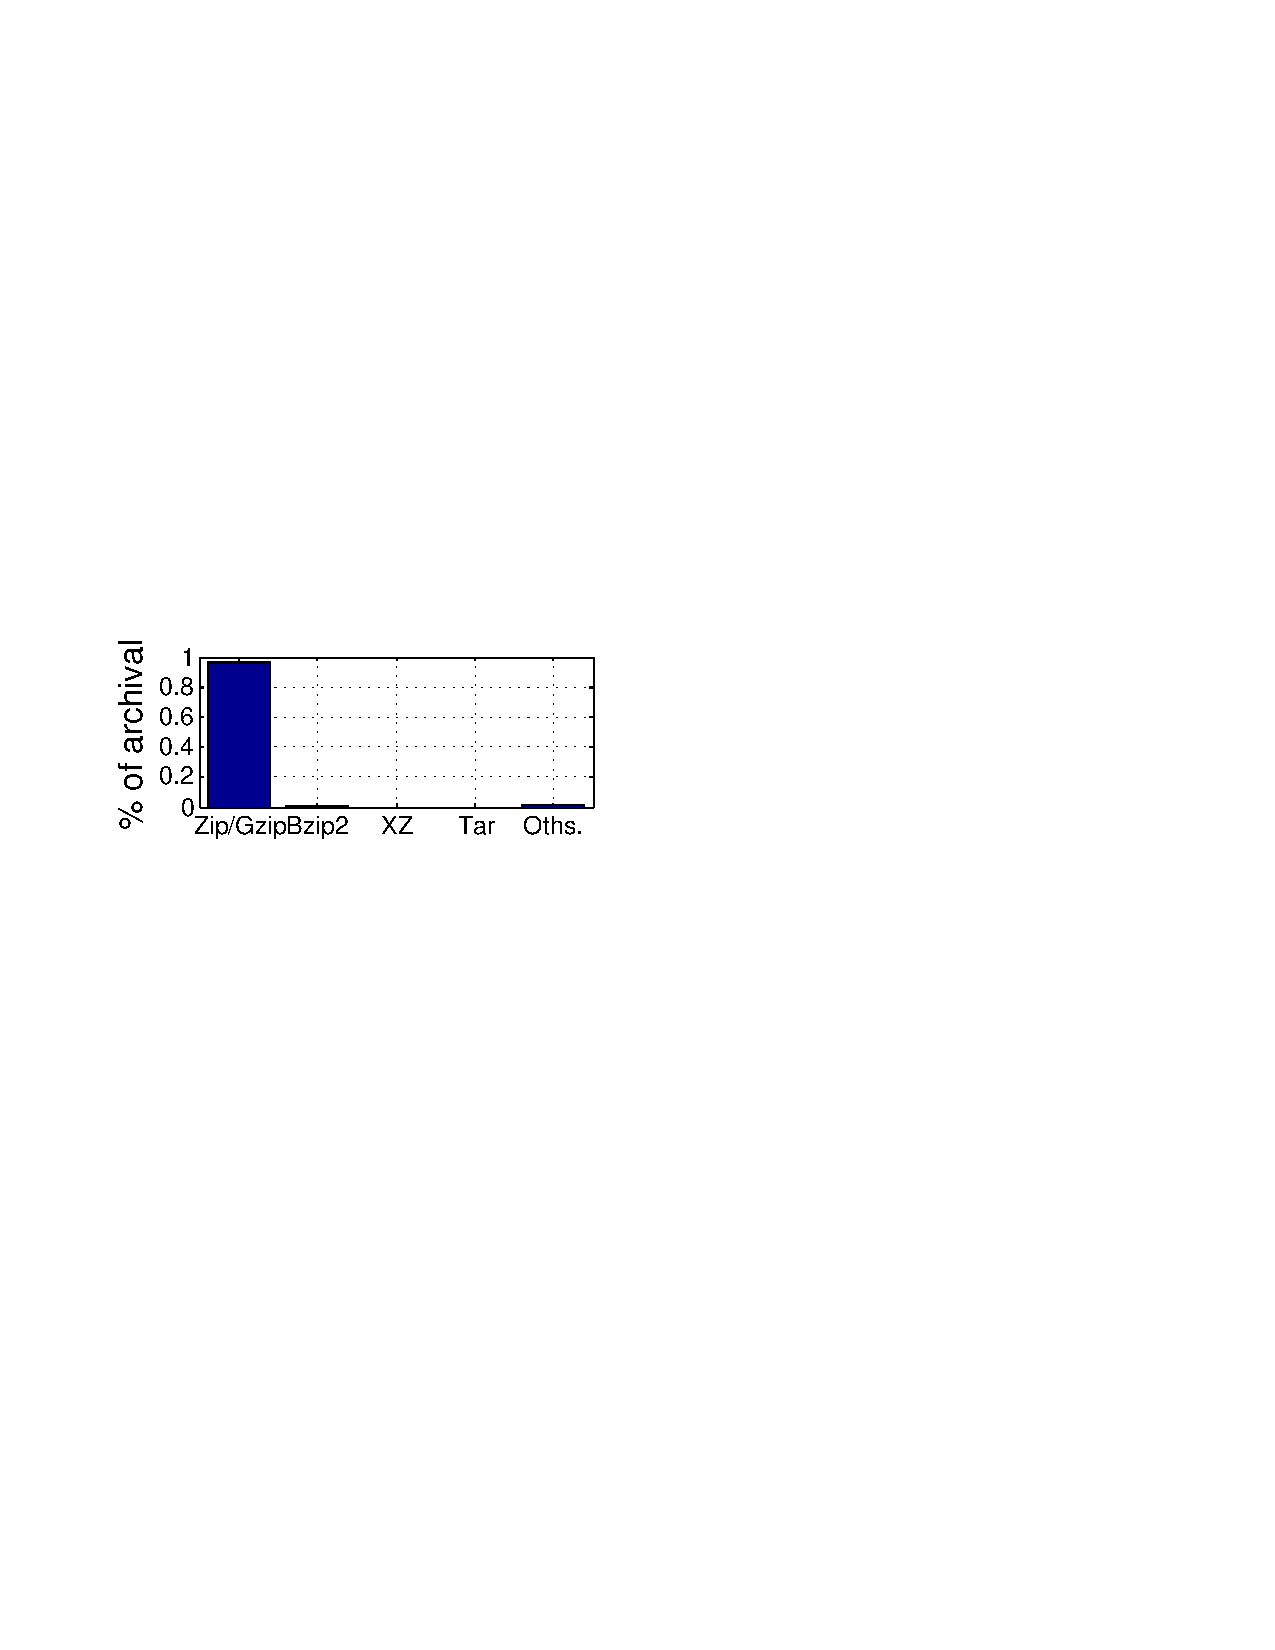
\includegraphics [width=0.22\textwidth]{graphs/type-arc-cnt}
	}
	\subfigure[Capacity (in \%) by file type.]{\label{fig:type-arc-size}
		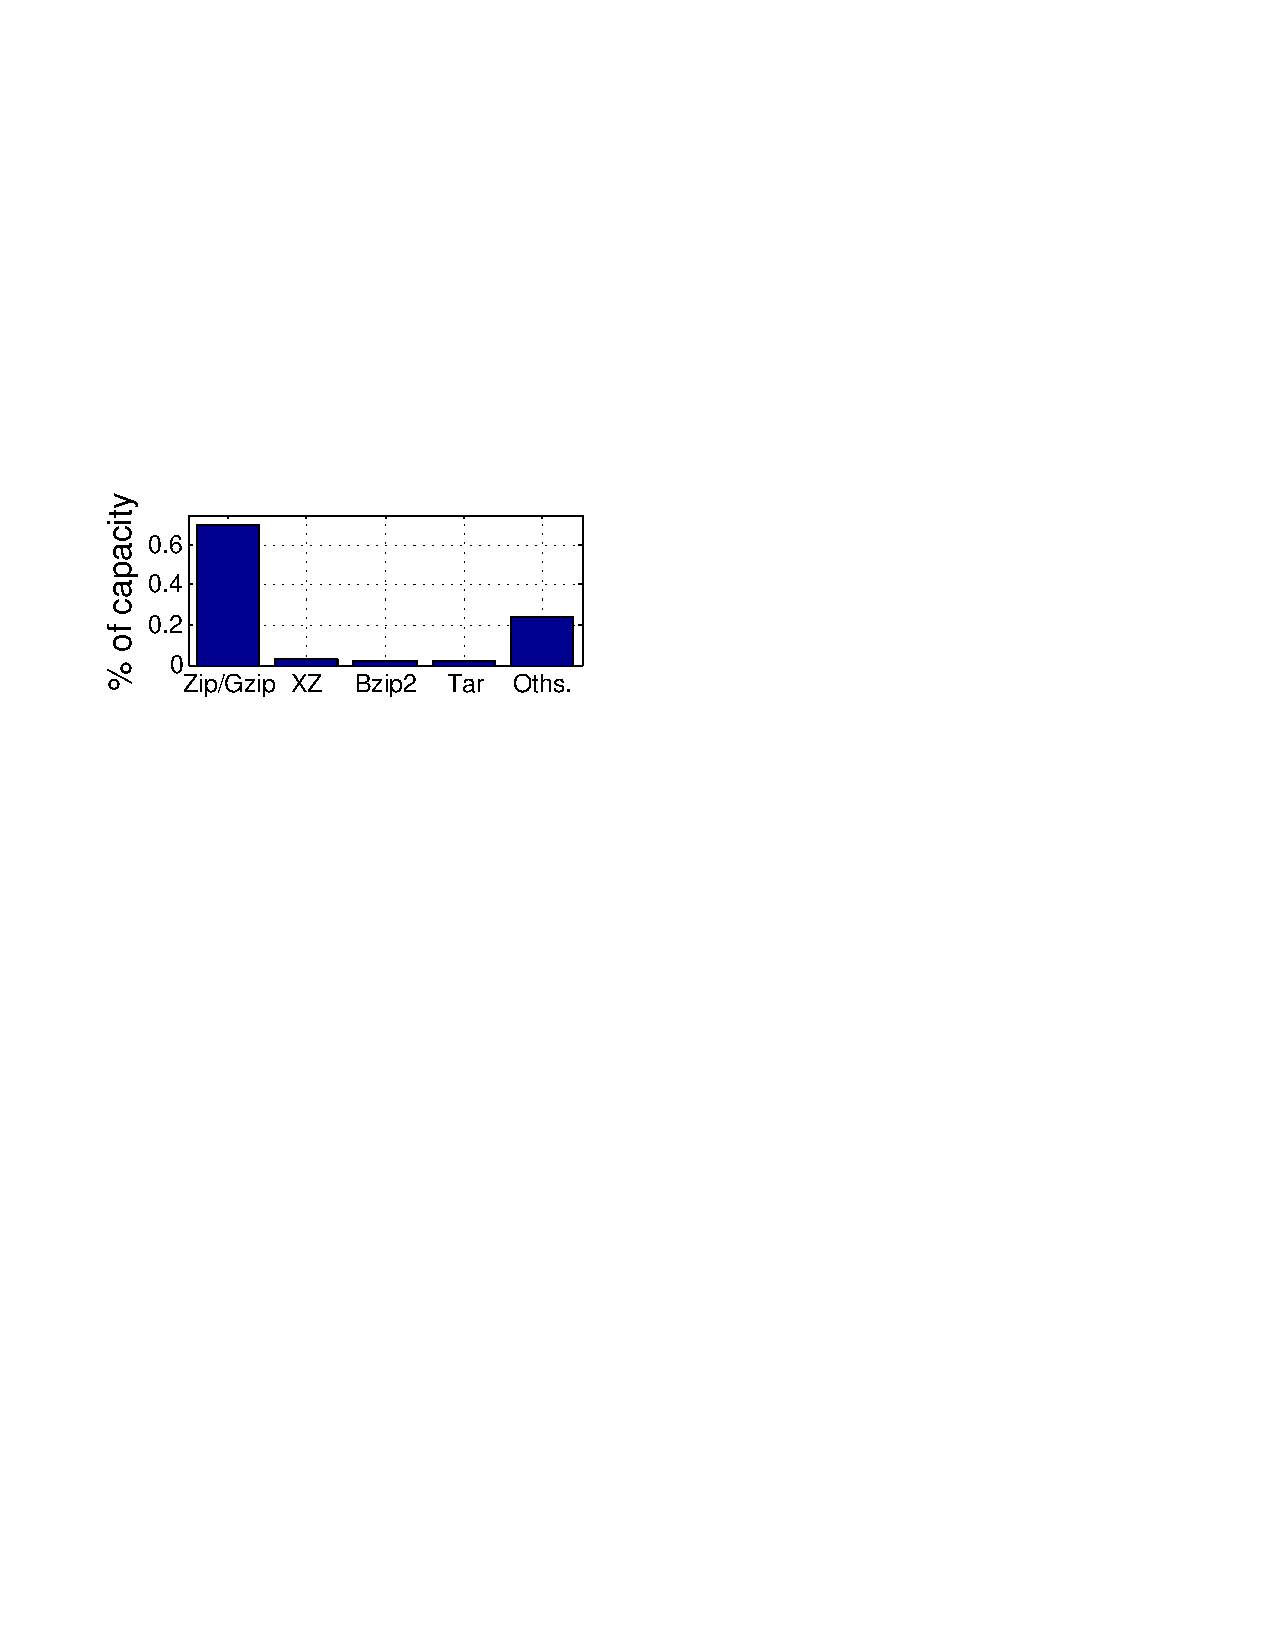
\includegraphics [width=0.22\textwidth]{graphs/type-arc-size}
	}
	\caption{Archival}
	\label{fig:arc-doc}
\end{figure} 

\paragraph{Databases (DB.)}

Interestingly, we found plenty of database related files in our dataset as currently there is a debate about whether we should run a database inside a container or not~\cite{xxx}. As shown in Figure~\ref{fig:arc-db}, we see that over half of database related files are Berkely DB (33\%) and MySQL (30\%) related files, but these two database related files take less than 40\% of capacity occupied by database related files. 7\% of database related files are SQLite DB files, which take up over 57\% of capacity occupied by database related files. 
%Database related files have the highest average file size.

\textit{We conclude that Docker developers run databases inside Docker containers. Most frequently used databases are Berkeley DB and MySQL, but they take less storage space. Most commonly used database (in terms of capacity) by Docker developer is SQLite DB.}

\begin{figure}
	\centering
	\subfigure[File count (in \%) by file type.]{\label{fig:type-db-cnt}
		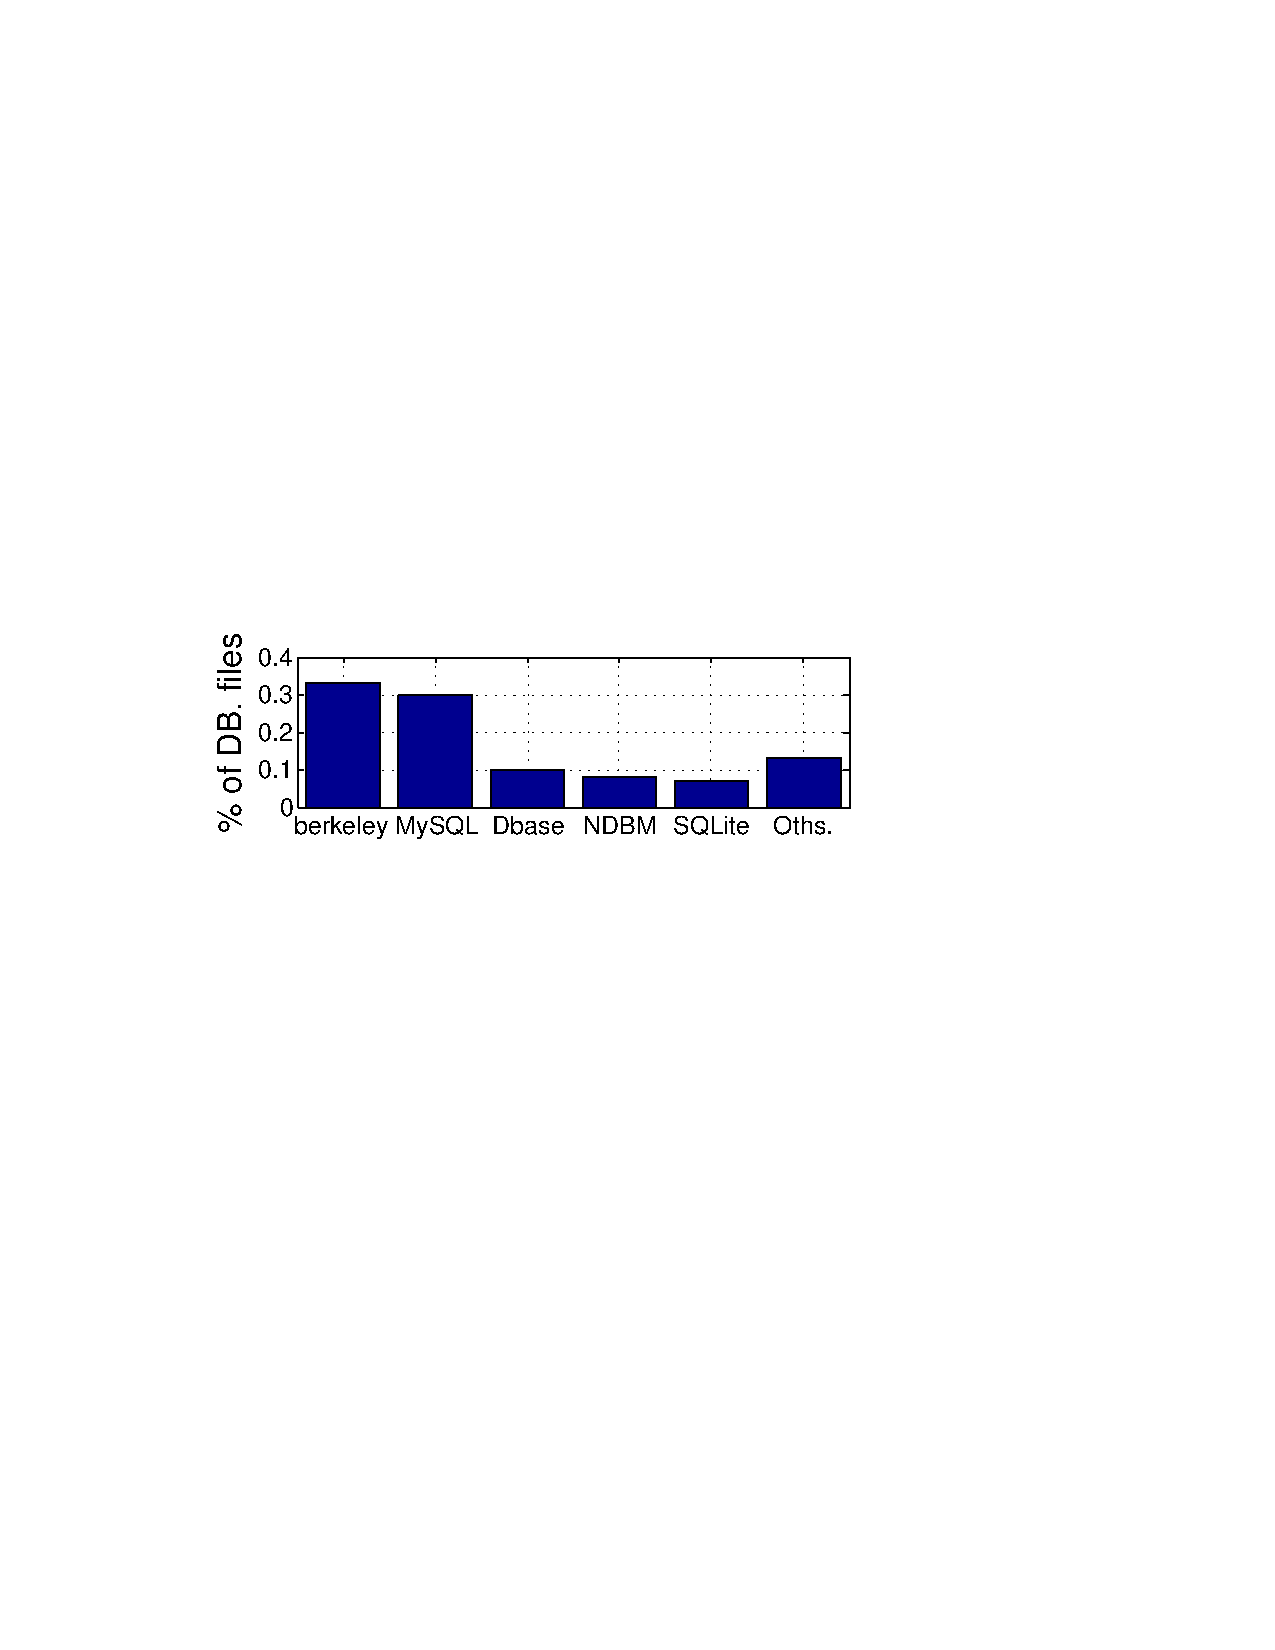
\includegraphics [width=0.225\textwidth]{graphs/type-db-cnt}
	}
	\subfigure[Capacity (in \%) by file type.]{\label{fig:type-db-size}
		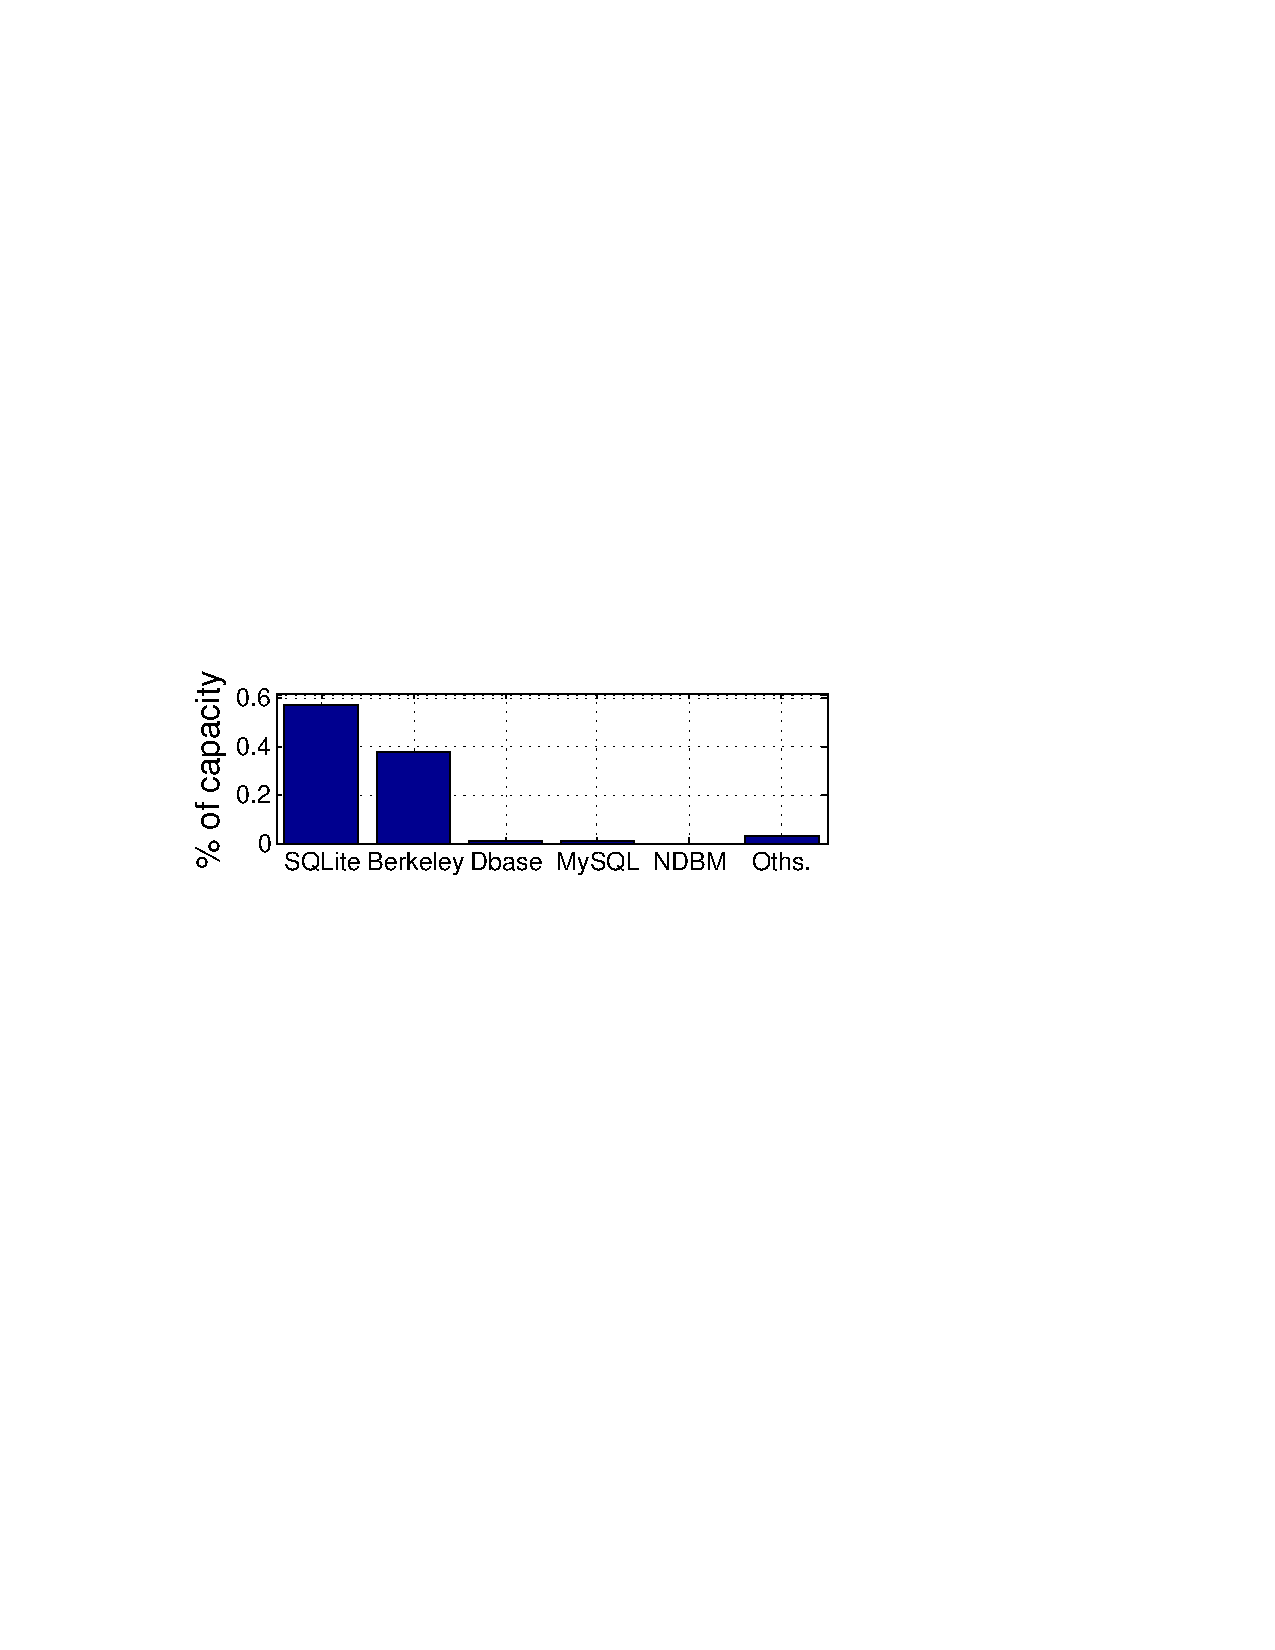
\includegraphics [width=0.225\textwidth]{graphs/type-db-size}
	}
	\caption{Databases}
	\label{fig:arc-db}
\end{figure} 

\paragraph{Images (Img.)}

Interestingly, Docker developers process image data files in Docker contains as we found plenty of image data files, such as PNG, JPEG, SVG, etc., although it requires efforts to run GUI applications inside containers.
As shown in figure~\ref{xxx}, more than half of image files are PNG files (67\%), which take up to 45\% of capacity occupied by image files. The second most commonly used image files are JPEG files which take up over 20\% capacity occupied by image files.

\textit{We conclude that majority of commonly used image files are PNG files and there are different types of image data files stored in Docker container.}

\begin{figure}
	\centering
	\subfigure[File count (in \%) by file type.]{\label{fig:type-img-cnt}
		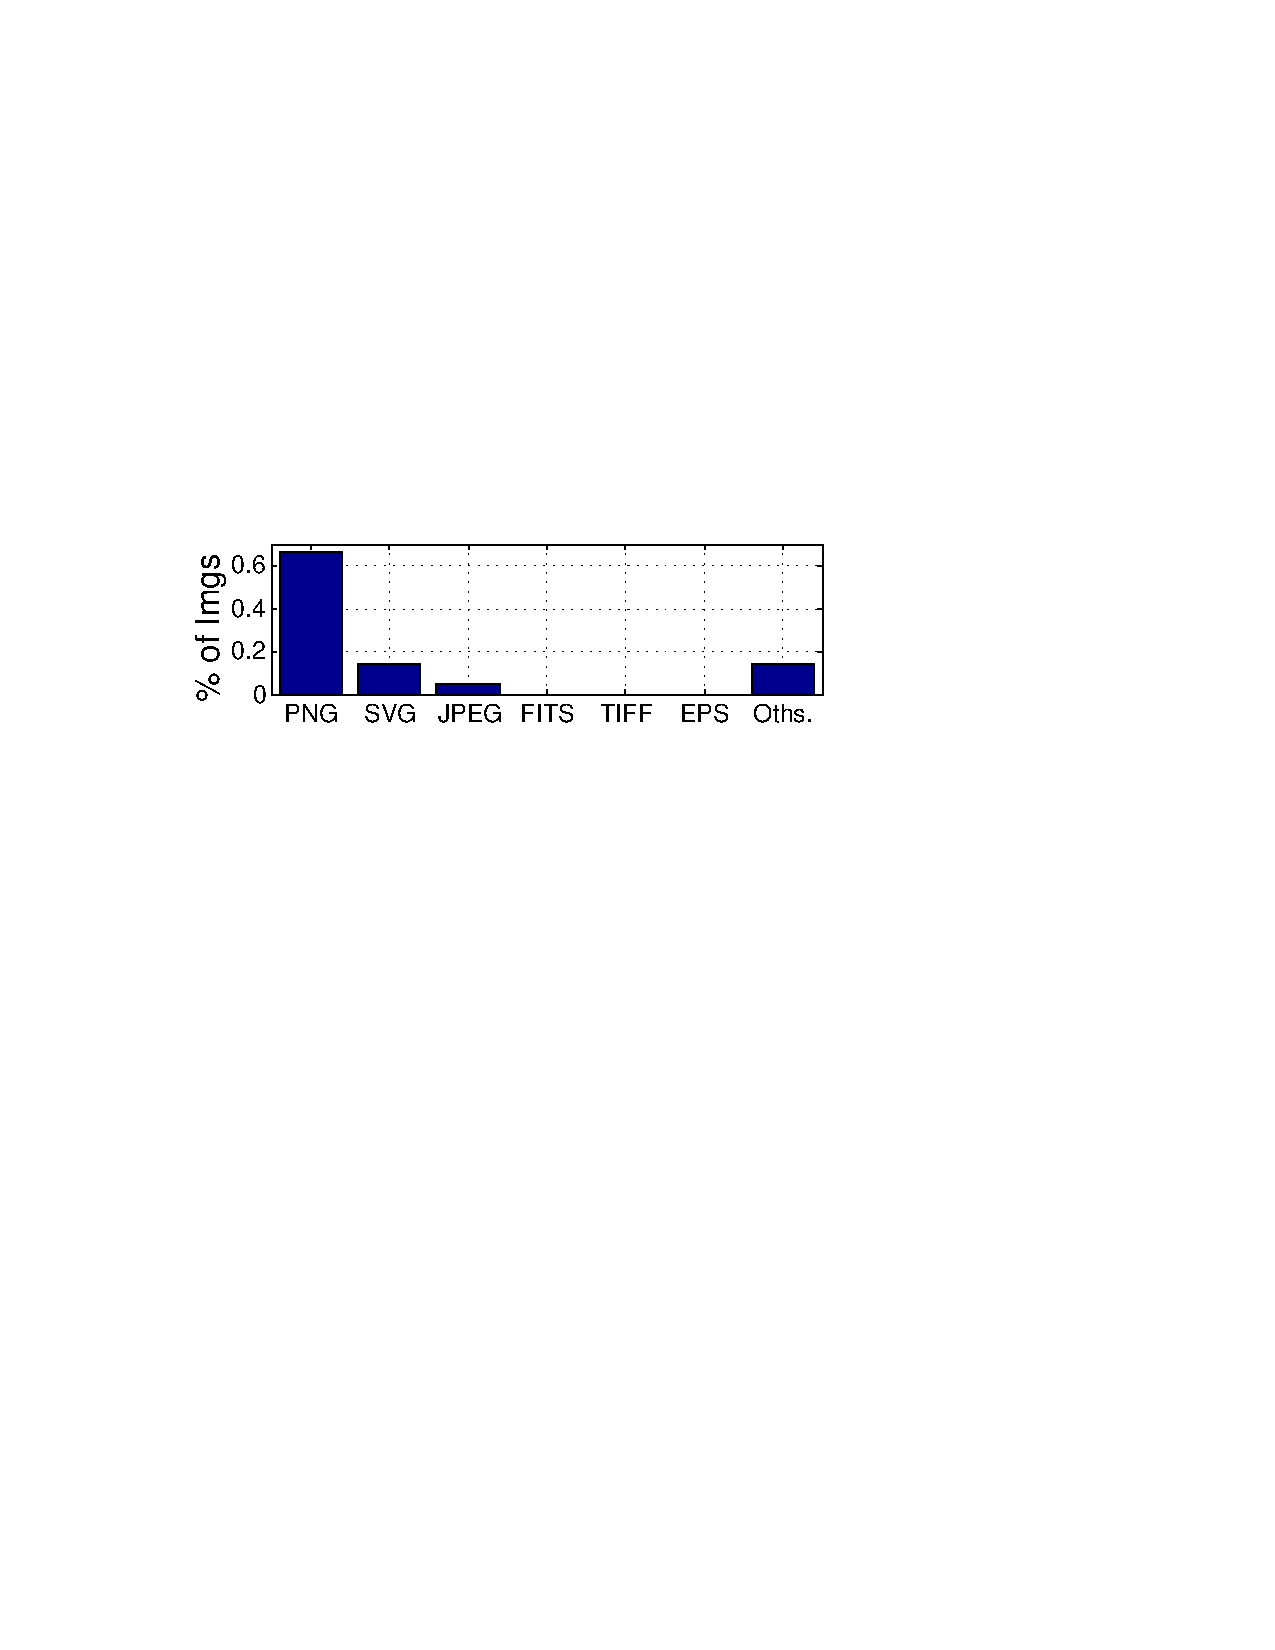
\includegraphics [width=0.225\textwidth]{graphs/type-img-cnt}
	}
	\subfigure[Capacity (in \%) by file type.]{\label{fig:type-img-size}
		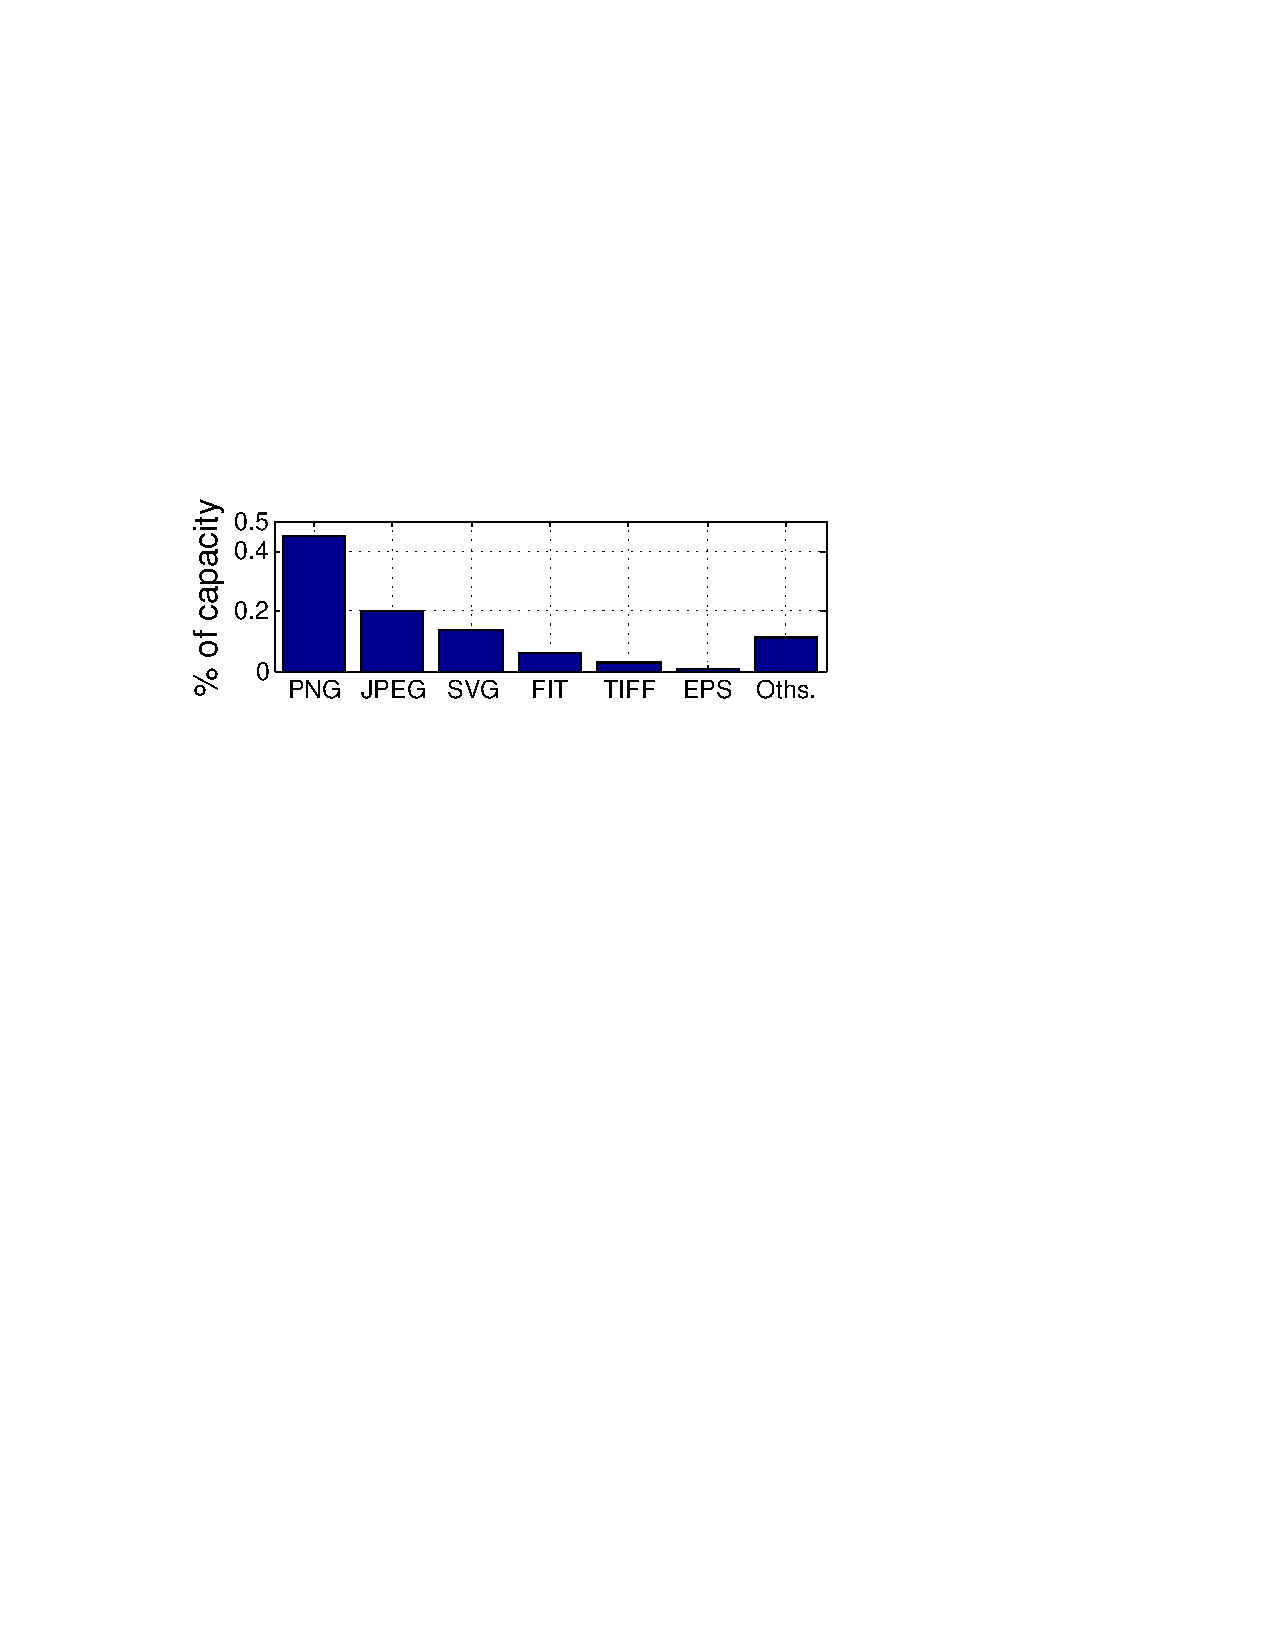
\includegraphics [width=0.225\textwidth]{graphs/type-img-size}
	}
	\caption{Images}
	\label{fig:arc-img}
\end{figure} 
%, , archival, images, databases, and others
%\paragraph{Overall file size}

%\begin{figure}
%	\centering
%	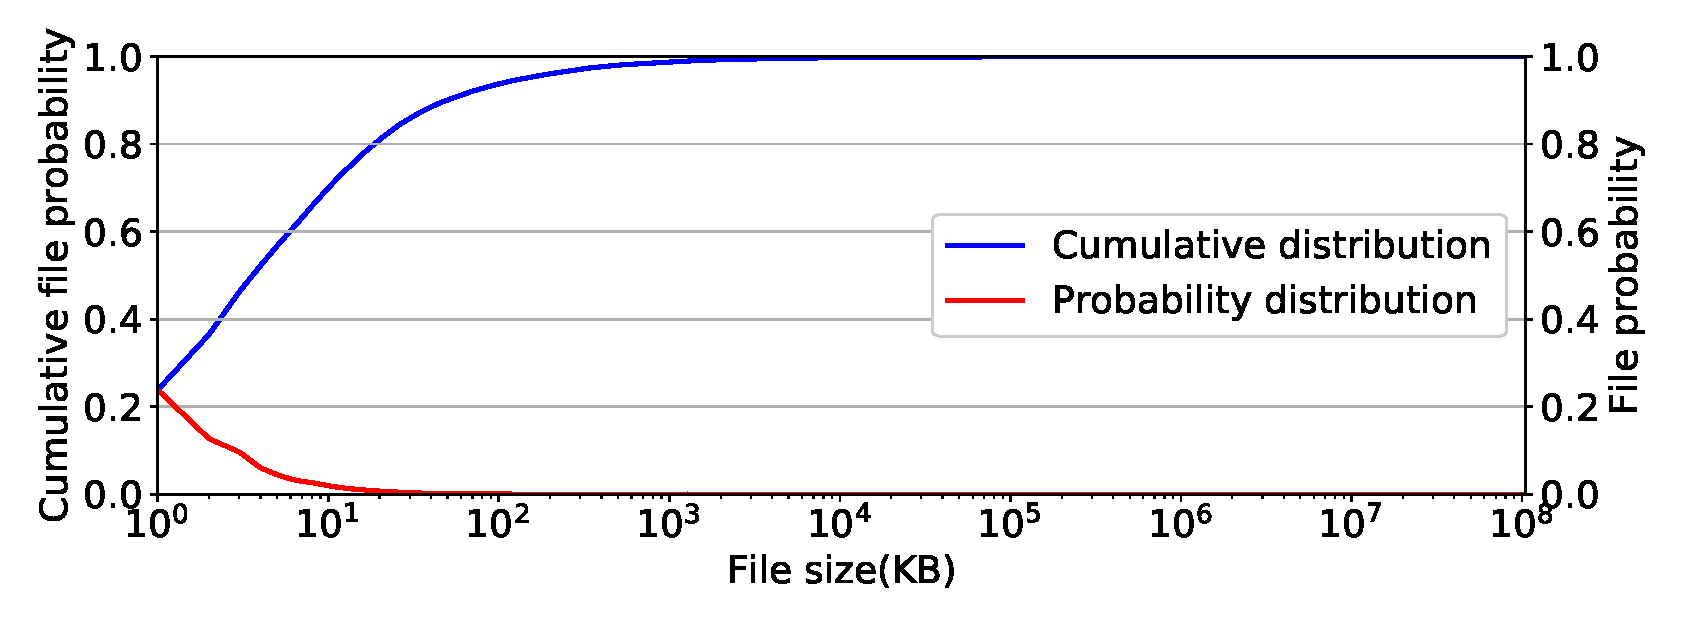
\includegraphics[width=0.5\textwidth]{graphs/File_size-KB.eps}
%	\caption{File size distribution.
%	}
%	\label{fig:file-size}
%\end{figure}
%
%Figure~\ref{fig:file-size} shows cumulative and probability distribution of file size.
%%of unique dataset after we remove the redundant files.
%\textit{Most files are smaller files.} For example, 91\% files are equal or less than 100 KB. 
%Around 22\% of files are less than 1 KB. 
%\textit{This is consistent with our finding that the layer size and image size are small both in compressed and uncompressed format.}  


%\subsection{File repeat count}
%\subsection{File size}


%As shown in Table~\ref{fig_image_growth}, the number of repositories increased
%linearly during our observation period from May 30th to September 20th,
%2017. Note that the graph shows a gap of 15 days due to Docker Hub changing the way it
%indexes repositories. The total number of repositories
%grew from 633,915 to 687,292, resulting in an average creation rate of 1,241
%repositories per day.
%This rapid growth of repositories suggests that storage optimizations will
%be crucial for registries in the neear future.
%Notice also,
%that each repository contains multiple tagged images and, therefore, we 
%significantly underestimatet the size of Docker Hub's content.
